\documentclass[a4paper,titlepage,12pt]{scrartcl}	%El modo de documento es para la numeración.

\usepackage{graphicx} %Imágenes
\usepackage[utf8]{inputenc} %Tildes
\usepackage[spanish,es-tabla]{babel} %Español, es-table: llamar tablas en vez de cuadros
\usepackage[breaklinks=true]{hyperref} %Hiperenlaces
\usepackage{amssymb, amsmath, amsbsy} %Símbolos matemáticos
\usepackage{float} %Mover las imágenes usando [H]
\usepackage{eurosym} %Símbolo de euro \euro
\usepackage{listings} %Código

\numberwithin{figure}{section} %Hace que la primera figura de cada sección X sea X.1
\numberwithin{table}{section} %Hace que la primera tabla de cada sección X sea X.1

\begin{document}
	\begin{titlepage}
		\begin{center}
			\begin{figure}[htb]
				\begin{center}
					
\includegraphics[width=12cm]{./Portada/ugr.png}
				\end{center}
			\end{figure}

			\vspace*{0.8cm}
			\begin{Large}
				\textbf{Grado en Ingeniería Informática.}\\
			\end{Large}
			\begin{Huge}
				\vspace{1.5cm}
				\textbf{Práctica 2.} \\
			\end{Huge}
			\vspace*{0.76cm}
			\rule{100mm}{0.1mm}\\
			\vspace*{0.5cm}
			\begin{large}
				\textbf{Nombre de la asignatura:}\\
				Ingeniería de Servidores.\\
				\vspace*{0.5cm}
				\textbf{Realizado por:}\\
				Néstor Rodríguez Vico \\

				\vspace*{2cm}
				\begin{figure}[htb]
					\begin{center}
						
\includegraphics[width=5cm]{./Portada/etsiit.png}
					\end{center}
				\end{figure}
				\vspace*{-0.6cm}
				ESCUELA TÉCNICA SUPERIOR DE INGENIERÍAS INFORMÁTICA Y DE TELECOMUNICACIÓN.\\
				\rule{20mm}{0.1mm}\\
				\vspace*{0.6cm}
				Granada, \today.
			\end{large}
		\end{center}
	\end{titlepage}
	
	%--------------Indices--------------
	\tableofcontents
	\clearpage
	\listoffigures %Imagenes
	\clearpage
	%----------------------------------
	
	%%%%%%%%%%%%%%%%%%%%%%%%%%%%%%%%%%%%%%%%%%%%%%%%%%%%
	%%%%%%%%%%%%%%%%%%%% Cuestión 1 %%%%%%%%%%%%%%%%%%%%
	%%%%%%%%%%%%%%%%%%%%%%%%%%%%%%%%%%%%%%%%%%%%%%%%%%%%	
	\section[Cuestión 1:]{Cuestión 1:}
	
	\subsection[a) Liste los argumentos de yum necesarios para instalar, buscar y eliminar paquetes.]{a) Liste los argumentos de yum necesarios para instalar, buscar y eliminar paquetes.}
	
	Como podemos ver en la página de RedHat \cite{yum}, los comandos son los siguientes:
	\begin{itemize}
		\item Instalar paquetes: \textit{yum install $<$nombre del paquete/s$>$}
		\item Buscar paquetes: \textit{yum search $<$palabra clave$>$}
		\item Eliminar paquetes: \textit{yum remove $<$nombre del paquete/s$>$}
	\end{itemize}
	
	Por lo tanto los argumentos son:
	\begin{itemize}
		\item Instalar paquetes: \textit{install}
		\item Buscar paquetes: \textit{search}
		\item Eliminar paquetes: \textit{remove}
	\end{itemize} 
	
	\subsection[b) ¿Qué ha de hacer para que yum pueda tener acceso a Internet en el PC del aula?(Pistas: archivo de configuración en /etc, proxy: stargate.ugr.es:3128).]{b) ¿Qué ha de hacer para que yum pueda tener acceso a Internet en el PC del aula?(Pistas: archivo de configuración en /etc, proxy: stargate.ugr.es:3128).}
	
	Para tener acceso a Internet, tenemos que configurar un proxy. Según CentOS \cite{yumproxy} hay que indicar el proxy en el archivo \textit{/etc/yum.conf}. Para tener acceso desde los ordenadores de la UGR, debemos añadir la siguiente línea: \textit{proxy=http://astargate.ugr.es:3128}
	
	Una manera de comprobar si funciona correctamente es añadir el proxy en mi ordenador. Si hacemos esto, al ejecutar por ejemplo \textit{sudo yum install httd} nos da error. Da error porque intenta conectarse hacia afuera usando ese proxy. De esta manera podemos ver que funciona correctamente. En la figura \ref{2-yum-proxy} podemos ver el error que obtenemos y como, efectivamente, está el proxy activado.
	
	\begin{figure}[H]
		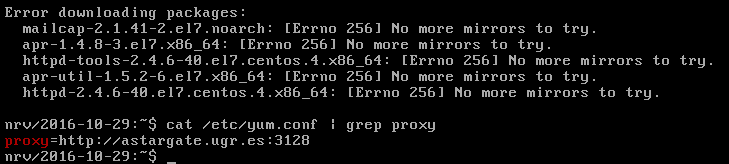
\includegraphics[width=\linewidth]{./Imagenes/2-yum-proxy.png}
		\vspace{-0.5cm}
		\caption[Error con el proxy añadido en mi ordenador (yum).]{Error con el proxy añadido en mi ordenador (yum).}
		\label{2-yum-proxy}
	\end{figure}
	
	\subsection[c) ¿Cómo añadimos un nuevo repositorio?]{c) ¿Cómo añadimos un nuevo repositorio?}
	
	Como podemos ver en la página de Centos \cite{yumproxy} para añadir un repositorio tenemos que ubicar el archivo de definiciones en el directorio \textit{/etc/yum.repos.d/}. Los proveedores de paquetes ponen los archivos de definiciones en sus páginas web. para añadir un archivo de definiciones hay que tener acceso root. Para copiar el archivo en textit{/etc/yum.repos.d/} debemos ejecutar el comando \textit{su -c 'cp example.repo /etc/yum.repos.d/'}.

	%%%%%%%%%%%%%%%%%%%%%%%%%%%%%%%%%%%%%%%%%%%%%%%%%%%%
	%%%%%%%%%%%%%%%%%%%% Cuestión 2 %%%%%%%%%%%%%%%%%%%%
	%%%%%%%%%%%%%%%%%%%%%%%%%%%%%%%%%%%%%%%%%%%%%%%%%%%%
	\section[Cuestión 2:]{Cuestión 2:}
	
	\subsection[a) Liste los argumentos de apt necesarios para instalar, buscar	y eliminar paquetes.]{a) Liste los argumentos de apt necesarios para instalar, buscar y eliminar paquetes.}
	
	En la página de Ubuntu \cite{apt} podemos ver los comandos para realizar las distintas tareas:
	\begin{itemize}
		\item Instalar paquetes: \textit{sudo apt-get install $<$nombre del paquete/s$>$}
		\item Buscar paquetes: \textit{apt-cache search $<$palabra clave$>$}
		\item Eliminar paquetes: \textit{sudo apt-get remove $<$nombre del paquete/s$>$}
	\end{itemize}
	
	Por lo tanto los argumentos son:
	\begin{itemize}
		\item Instalar paquetes: \textit{install}
		\item Buscar paquetes: \textit{search}
		\item Eliminar paquetes: \textit{remove}
	\end{itemize} 
	
	Nota: \textit{-get} y \textit{-cache} no son necesarios en la versiones más modernas de \textit{apt}.
	
	\subsection[b)¿Qué ha de hacer para que apt pueda tener acceso a Internet en el PC del aula?(Pistas: archivo de configuración en /etc, proxy: stargate.ugr.es:3128)]{b)¿Qué ha de hacer para que apt pueda tener acceso a Internet en el PC del aula?(Pistas: archivo de configuración en /etc, proxy: stargate.ugr.es:3128)}
	
	Para tener acceso a Internet, tenemos que configurar un proxy. Según Ubuntu \cite{apt} hay que indicar el proxy en el archivo \textit{/etc/apt/apt.conf}. Para tener acceso desde los ordenadores de la UGR, hay que añadir la línea: \textit{Acquire::http::Proxy ``astargate.ugr.es:3128'';}
	
	Una manera de comprobar si funciona correctamente es añadir el proxy en mi ordenador. Si hacemos esto, al ejecutar por ejemplo \textit{sudo apt update} nos da error. Da error porque intenta conectarse hacia afuera usando ese proxy. De esta manera podemos ver que funciona correctamente. En la figura \ref{2-apt-proxy} podemos ver el error que obtenemos y como, efectivamente, está el proxy activado.
	
	\begin{figure}[H]
		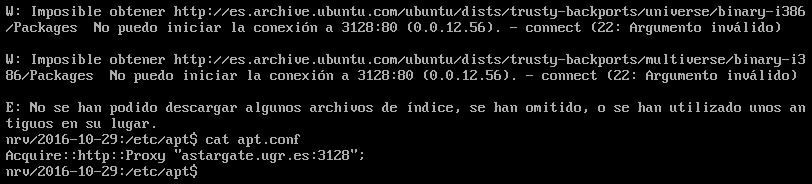
\includegraphics[width=\linewidth]{./Imagenes/2-apt-proxy.png}
		\vspace{-0.5cm}
		\caption[Error con el proxy añadido en mi ordenador (apt).]{Error con el proxy añadido en mi ordenador (apt).}
		\label{2-apt-proxy}
	\end{figure}
	
	\subsection[c)¿Cómo añadimos un nuevo repositorio?]{c)¿Cómo añadimos un nuevo repositorio?}
	
	Según Ubuntu \cite{aptrepo} hay dos maneras de hacerlo:
	\begin{itemize}
		\item Si el repositorio se encuentra en el fichero \textit{/etc/apt/sources.list}, tenemos que descomentarlo, es decir, quitar el símbolo \textit{\#} que precede a las líneas correspondientes al repositorio o ejecutando la orden \textit{sudo add-apt-repository $<$repositorio a añadir$>$}
		\item Si el repositorio es PPA, debemos ejecutar la orden \textit{sudo add-apt-repository ppa:$<$nombre del repositorio$>$}
	\end{itemize}
	
	%%%%%%%%%%%%%%%%%%%%%%%%%%%%%%%%%%%%%%%%%%%%%%%%%%%%
	%%%%%%%%%%%%%%%%%%%% Cuestión 3 %%%%%%%%%%%%%%%%%%%%
	%%%%%%%%%%%%%%%%%%%%%%%%%%%%%%%%%%%%%%%%%%%%%%%%%%%%
	\section[Cuestión 3:]{Cuestión 3:}
	
	\subsection[a) ¿Con qué comando puede abrir/cerrar un puerto usando ufw? Muestre un ejemplo de cómo lo ha hecho.]{a) ¿Con qué comando puede abrir/cerrar un puerto usando ufw? Muestre un ejemplo de cómo lo ha hecho.}
	
	Cómo podemos ver en la página de Ubuntu \cite{ufw_puertos}, podemos usar los siguientes comandos para abrir y cerrar puertos, ambos deben ser ejecutado como \textit{root}:
	\begin{itemize}
		\item Abrir un puerto: \textit{ufw allow $<$puerto$>$/$<$opcional: protocolo$>$}
		\item Cerrar un puerto: \textit{ufw deny $<$puerto$>$/$<$opcional: protocolo$>$}
	\end{itemize}
	
	\subsection[b) ¿Con qué comando puede abrir/cerrar un puerto usando firewall-cmd en CentOS? Muestre un ejemplo de cómo lo ha hecho.]{b) ¿Con qué comando puede abrir/cerrar un puerto usando firewall-cmd en CentOS? Muestre un ejemplo de cómo lo ha hecho.}
	
	Cómo podemos ver en la página de RedHat \cite{firewall-cmd_puertosRH} y en la de Fedora \cite{firewall-cmd_puertosFedora}, podemos usar los siguientes comandos para abrir y cerrar puertos, ambos deben ser ejecutado como \textit{root}:
	\begin{itemize}
		\item Abrir un puerto: \textit{firewall-cmd [{-}-zone=$<$zona$>$] {-}-add-port=$<$puerto$>$/$<$protocolo$>$}
		\item Cerrar un puerto: \textit{firewall-cmd [{-}-zone=$<$zona$>$] {-}-remove-port=$<$puerto$>$/$<$protocolo$>$}
	\end{itemize}
	
	\subsection[c) Utilice el comando nmap para ver que, efectivamente, los puertos están accesibles.]{c) Utilice el comando nmap para ver que, efectivamente, los puertos están accesibles.}
	
	Para entender los resultados que nos devuelve nmap lo mejor es ver la página de ellos \cite{nmap}. Hay que tener especial cuidado con el estado \textit{closed}, ya que cómo podemos ver en la página de nmap puede haber puertos abiertos pero que no hay ningún programa escuchando dicho puerto y por lo tanto el estado de dicho puerto es \textit{closed}. En ambos sistemas operativos (Ubuntu Server y CentOS) voy a abrir el puerto 10.
	
	\begin{figure}[H]
		\centering
		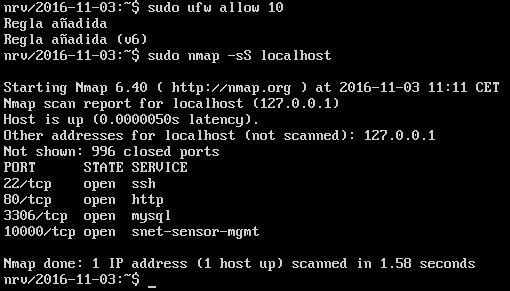
\includegraphics[scale=0.82]{./Imagenes/3-nmapubuntu.png}
		\caption[Puerto 10 habilitado y análisis de los puertos con nmap (Ubuntu Server).]{Puerto 10 habilitado y análisis de los puertos con nmap (Ubuntu Server).}
		\label{3-nmapubuntu}
	\end{figure}
	
	\begin{figure}[H]
		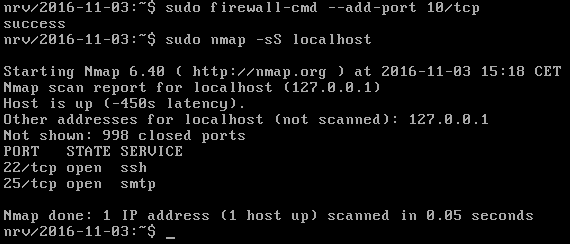
\includegraphics[width=\linewidth]{./Imagenes/3-nmapcentos.png}
		\vspace{-0.5cm}
		\caption[Puerto 10 habilitado y análisis de los puertos con nmap (Ubuntu Server).]{Puerto 10 habilitado y análisis de los puertos con nmap (Ubuntu Server).}
		\label{3-nmapcentos}
	\end{figure}
	
	Como podemos ver, ni en la figura \ref{3-nmapubuntu} ni en la figura \ref{3-nmapcentos} aparece el puerto abierto tras la ejecución del comando \textit{sudo nmap -sS localhost} pero están abiertos correctamente. Esto se debe a la explicación anterior.
	
	%%%%%%%%%%%%%%%%%%%%%%%%%%%%%%%%%%%%%%%%%%%%%%%%%%%%
	%%%%%%%%%%%%%%%%%%%% Cuestión 4 %%%%%%%%%%%%%%%%%%%%
	%%%%%%%%%%%%%%%%%%%%%%%%%%%%%%%%%%%%%%%%%%%%%%%%%%%%	
	\section[Cuestión 4: ¿Qué diferencia hay entre telnet y ssh?]{Cuestión 4: ¿Qué diferencia hay entre telnet y ssh?}
	
	Comparando las páginas de Telnet \cite{telnet} y la de OpenSHH \cite{openssh} podemos ver que la mayor diferencia reside en la seguridad. ssh cifra los datos para mantener la comunicación segura mientras que telnet no.
	
	%%%%%%%%%%%%%%%%%%%%%%%%%%%%%%%%%%%%%%%%%%%%%%%%%%%%
	%%%%%%%%%%%%%%%%%%%% Cuestión 5 %%%%%%%%%%%%%%%%%%%%
	%%%%%%%%%%%%%%%%%%%%%%%%%%%%%%%%%%%%%%%%%%%%%%%%%%%%
	\section[Cuestión 5:]{Cuestión 5:}
	
	\subsection[a) ¿Para qué sirve la opción -X?]{a) ¿Para qué sirve la opción -X?}
	
	Como podemos ver en las páginas de manual de ssh \cite{opensshman}, la opción -X sirve para activar el reenvío X11.
	
	\subsection[b) Ejecute remotamente, es decir, desde la máquina anfitriona (si tiene Linux) o desde la otra máquina virtual, el comando gedit en una sesión abierta con ssh. ¿Qué ocurre?]{b) Ejecute remotamente, es decir, desde la máquina anfitriona (si tiene Linux) o desde la otra máquina virtual, el comando gedit en una sesión abierta con ssh. ¿Qué ocurre?}
	
	\begin{figure}[H]
		\centering
		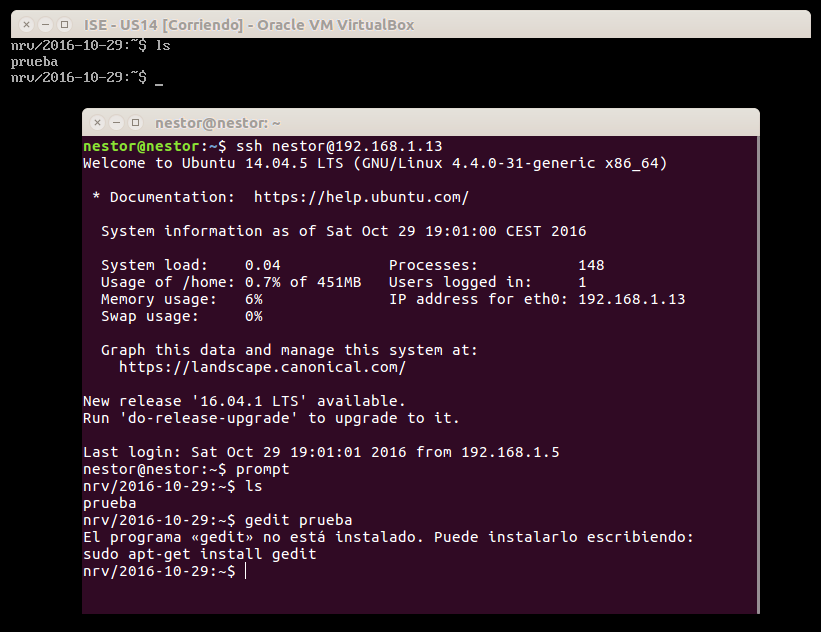
\includegraphics[scale=0.43]{./Imagenes/5-gedit.png}
		\caption[Error al ejecutar gedit en remoto (máquinas conectadas en modo \textit{bridge}).]{Error al ejecutar gedit en remoto (máquinas conectadas en modo \textit{bridge}).}
	\end{figure}
	
	El error se debe a que gedit no se encuentra instalado en Ubuntu Server y por eso no se puede ejecutar. Para instalarlo ejecutamos \textit{sudo apt install gedit}. Una vez instalado, probamos de nuevo a ejecutar \textit{gedit prueba} pero nos sigue dando error, como podemos ver en la figura \ref{5-errorgedit}.
	
	\begin{figure}[H]
		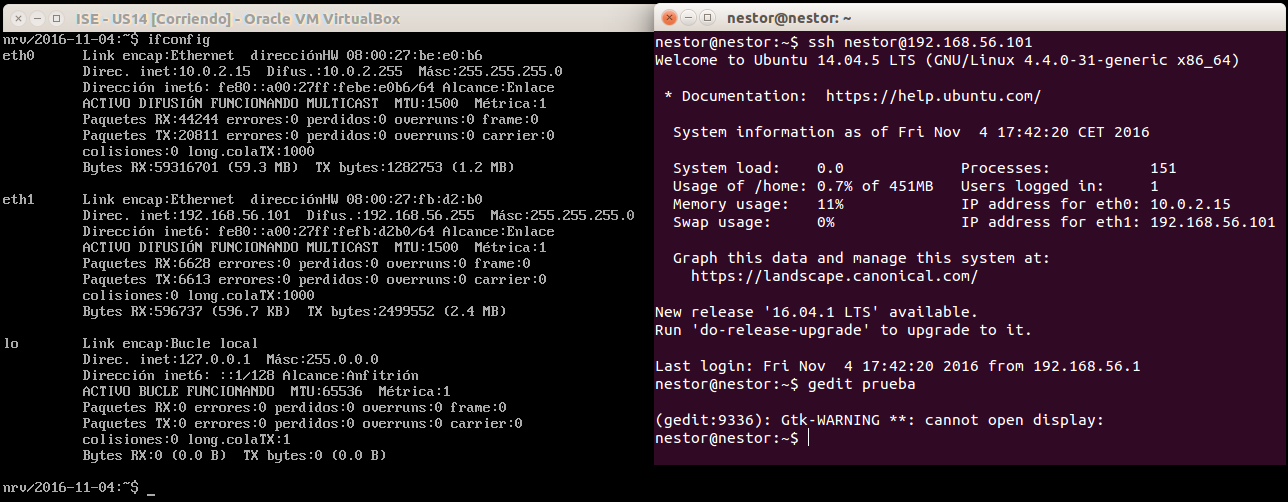
\includegraphics[width=\linewidth]{./Imagenes/5-errorgedit.png}
		\vspace{-0.5cm}
		\caption[Error tras instalar gedit en remoto (máquinas conectadas en modo \textit{bridge}).]{Error tras instalar gedit en remoto (máquinas conectadas en modo \textit{bridge}).}
		\label{5-errorgedit}
	\end{figure}
	
	Para arreglarlo, debemos conectarnos a ssh con el argumento -X, tal y como vimos en el apartado anterior de esta misma pregunta. Podemos ver que ahora si se abre gedit correctamente, como se ve en la figura \ref{5-geditfuncionando}.
	\begin{figure}[H]
		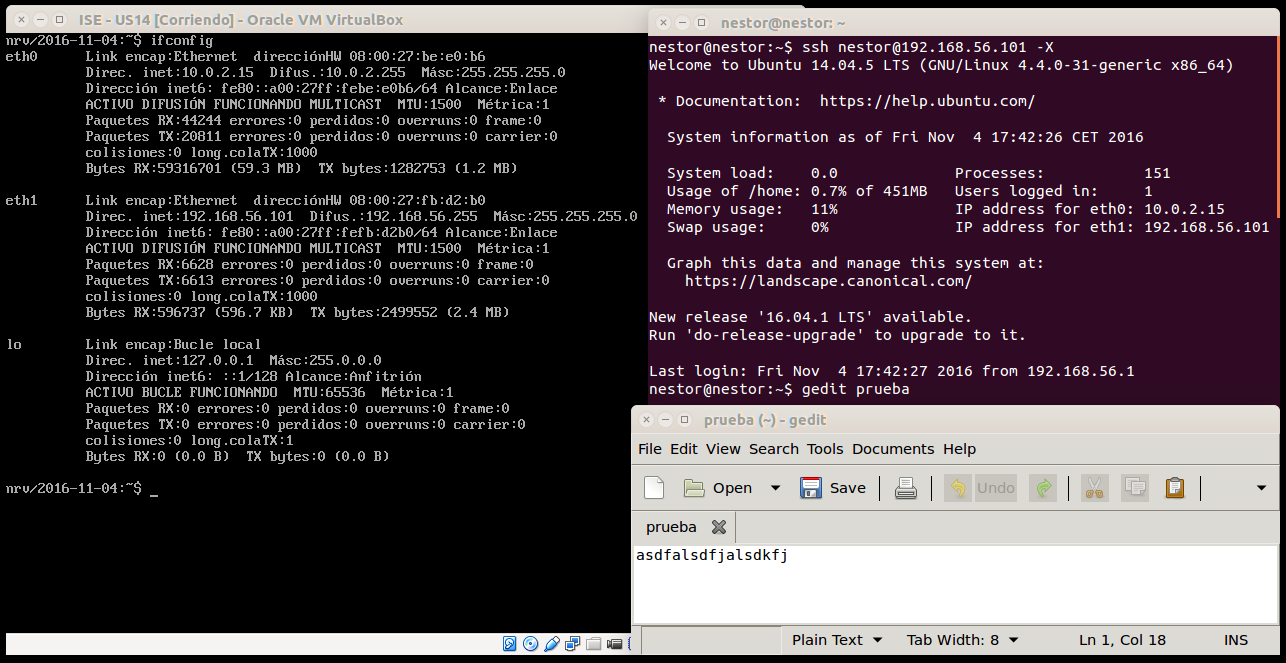
\includegraphics[width=\linewidth]{./Imagenes/5-geditfuncionando.png}
		\vspace{-0.5cm}
		\caption[gedit funcionando (máquinas conectadas en modo \textit{bridge}).]{gedit funcionando (máquinas conectadas en modo \textit{bridge}).}
		\label{5-geditfuncionando}
	\end{figure}
	
	%%%%%%%%%%%%%%%%%%%%%%%%%%%%%%%%%%%%%%%%%%%%%%%%%%%%
	%%%%%%%%%%%%%%%%%%%% Cuestión 6 %%%%%%%%%%%%%%%%%%%%
	%%%%%%%%%%%%%%%%%%%%%%%%%%%%%%%%%%%%%%%%%%%%%%%%%%%%
	\section[Cuestión 6: Muestre la secuencia de comandos y las modificaciones a los archivos correspondientes para permitir acceder a la consola remota sin introducir la contraseña. Pruebe que funciona. (Pistas: ssh-keygen, ssh-copy-id).]{Cuestión 6: Muestre la secuencia de comandos y las modificaciones a los archivos correspondientes para permitir acceder a la consola remota sin introducir la contraseña. Pruebe que funciona. (Pistas: ssh-keygen, ssh-copy-id).}
	
	Gracias a la información adquirida en la página de CentOS \cite{sshwithoutpswcentos} y en la página de Debian \cite{sshwithoutpswdebian}, los pasos que he seguido yo son:
	
	\begin{enumerate}
		\item Crear el par clave pública/clave privada en el cliente, en mi caso es mi ordenador, con el comando \textit{ssh-keygen -t rsa}
		\item Para mejorar la seguridad de el par de claves generadas, ejecutamos en el cliente el comando \textit{chmod 700 $\sim$/.ssh} y el comando \textit{chmod 600 $\sim$/.ssh/id\_rsa}
		\item Copiamos la llave pública generada en el servidor. El nombre de usuario de mi servidor es \textit{nestor} y la dirección IP es \textit{192.168.1.135}. Para copiar la llave pública ejecutamos desde el cliente \textit{ssh-copy-id -i $\sim$/.ssh/id\_rsa.pub nestor@192.168.1.13}
		\item Al igual que hicimos en el cliente, cambiamos los permisos de los archivos en el servidor ejecutando el comando \textit{chmod 700 $\sim$/.ssh} y el comando \textit{chmod 600 $\sim$/.ssh/id\_rsa}
	\end{enumerate}
	
	Siguiendo estos pasos, podemos conectarnos a nuestro servidor ssh sin tener que introducir las contraseña, como podemos ver en la figura \ref{6-ssh}:
	
	\begin{figure}[H]
		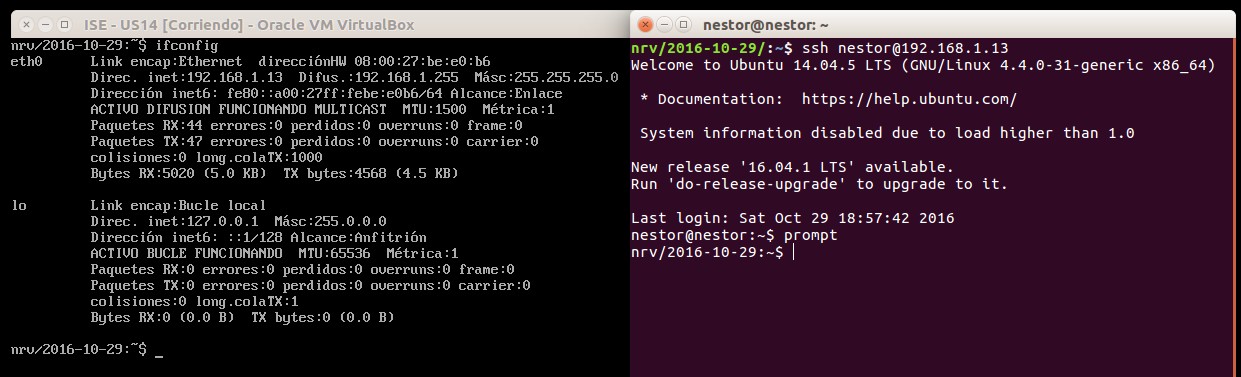
\includegraphics[width=\linewidth]{./Imagenes/6-ssh.png}
		\vspace{-0.5cm}
		\caption[Conexión ssh sin contraseña (máquinas conectadas en modo \textit{bridge}).]{Conexión ssh sin contraseña (máquinas conectadas en modo \textit{bridge}).}
		\label{6-ssh}
	\end{figure}
	
	%%%%%%%%%%%%%%%%%%%%%%%%%%%%%%%%%%%%%%%%%%%%%%%%%%%%
	%%%%%%%%%%%%%%%%%%%% Cuestión 7 %%%%%%%%%%%%%%%%%%%%
	%%%%%%%%%%%%%%%%%%%%%%%%%%%%%%%%%%%%%%%%%%%%%%%%%%%%
	\section[Cuestión 7: ¿Qué archivo es el que contiene la configuración del servicio ssh? ¿Qué parámetro hay que modificar para evitar que el usuario root acceda? Cambie el puerto por defecto y compruebe que puede acceder.]{Cuestión 7: ¿Qué archivo es el que contiene la configuración del servicio ssh? ¿Qué parámetro hay que modificar para evitar que el usuario root acceda? Cambie el puerto por defecto y compruebe que puede acceder.}
	
	El archivo que tiene la configuración del servicio ssh es \textit{/etc/ssh/sshd\_config}. \cite{opensshconfigman} \\
	
	Como podemos ver en las páginas de manual de \textit{sshd\_config} \cite{opensshconfigman} para evitar que el usuario acceda hay que cambiar el parámetro \textit{PermitRootLogin} que se encuentra en el archivo \textit{/etc/ssh/sshd\_config}. Inicialmente vemos \textit{PermitRootLogin without-password} y debemos escribir  \textit{PermitRootLogin no}. Una vez hecho el cambio, debemos reiniciar el servico con \textit{sudo service ssh restart}. Como podemos ver en la figura \ref{7-noroot} no se permite la conexión al usuario root.
	\begin{figure}[H]
		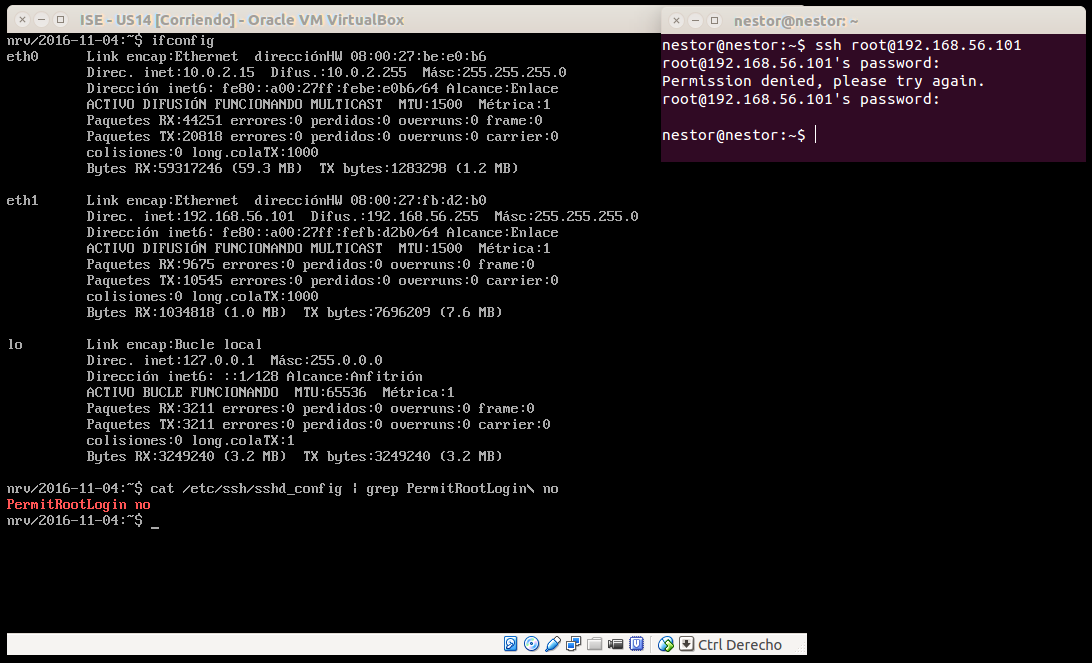
\includegraphics[width=\linewidth]{./Imagenes/7-noroot.png}
		\vspace{-0.5cm}
		\caption[Conexión no permitida al usuario root (máquinas conectadas en modo \textit{host-only}).]{Conexión no permitida al usuario root (máquinas conectadas en modo \textit{host-only}).}
		\label{7-noroot}
	\end{figure}
	
	Como podemos ver en las páginas de manual de \textit{sshd\_config} \cite{opensshconfigman} para cambiar el puerto por defecto hay que cambiar el parámetro \textit{Port} que se encuentra en \textit{/etc/ssh/sshd\_config}. Inicialmente vemos \textit{Port 22} y debemos escribir  \textit{Port $<$puerto\_deseado$>$}. Una vez hecho el cambio, debemos reiniciar el servico con \textit{sudo service ssh restart}. Ahora, para acceder debemos indicar el puerto con la opción \textit{-p}. La orden para conectarnos sería \textit{ssh -p puerto usuario@dirección}. Yo he cambiado el puerto 22 por el puerto 23 como podemos ver en la figura \ref{7-puerto}. Puedo seguir conectándome como podemos ver en la figura \ref{7-puerto}.
	
	\begin{figure}[H]
		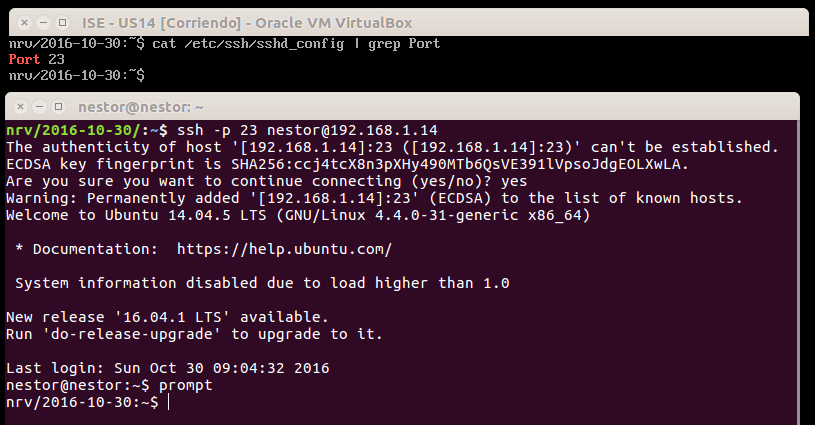
\includegraphics[width=\linewidth]{./Imagenes/7-puerto.png}
		\vspace{-0.5cm}
		\caption[Conexión ssh con el puerto cambiado al puerto 23 (máquinas conectadas en modo \textit{bridge}).]{Conexión ssh con el puerto cambiado al puerto 23 (máquinas conectadas en modo \textit{bridge}).}
		\label{7-puerto}
	\end{figure}
	
	%%%%%%%%%%%%%%%%%%%%%%%%%%%%%%%%%%%%%%%%%%%%%%%%%%%%
	%%%%%%%%%%%%%%%%%%%% Cuestión 8 %%%%%%%%%%%%%%%%%%%%
	%%%%%%%%%%%%%%%%%%%%%%%%%%%%%%%%%%%%%%%%%%%%%%%%%%%%
	\section[Cuestión 8: Indique si es necesario reiniciar el servicio ¿Cómo se reinicia un servicio en Ubuntu? ¿y en CentOS? Muestre la secuencia de comandos para hacerlo.]{Cuestión 8: Indique si es necesario reiniciar el servicio ¿Cómo se reinicia un servicio en Ubuntu? ¿y en CentOS? Muestre la secuencia de comandos para hacerlo.}
	
	Es necesario reiniciar un servicio cada vez que se cambié algo de la configuración de dicho servicio. En caso de que no se reiniciase, los cambios no sería visible hasta el próximo reinicio. \\
	
	Para reiniciar un servicio hay que ejecutar un comando distinto según si estamos en Ubuntu \cite{restartUbuntu} o en CentOS \cite{restartcentos}:
	\begin{itemize}
		\item \textbf{Ubuntu (ver figura \ref{8-restartubuntu}):} \textit{sudo service nombre\_servicio restart}
		\item \textbf{CentOS (ver figura \ref{8-restartcentos}):} \textit{systemctl restart nombre\_servicio}
	\end{itemize}
	
	\begin{figure}[H]
		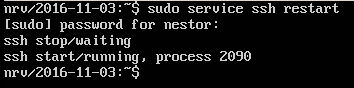
\includegraphics[width=\linewidth]{./Imagenes/8-restartubuntu.png}
		\vspace{-0.5cm}
		\caption[Reinicio del servicio ssh.]{Reinicio del servicio ssh.}
		\label{8-restartubuntu}
	\end{figure}
	
	\begin{figure}[H]
		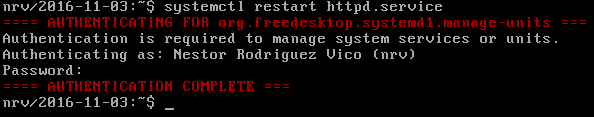
\includegraphics[width=\linewidth]{./Imagenes/8-restartcentos.png}
		\vspace{-0.5cm}
		\caption[Reinicio del servicio httpd.]{Reinicio del servicio httpd.}
		\label{8-restartcentos}
	\end{figure}
	
	%%%%%%%%%%%%%%%%%%%%%%%%%%%%%%%%%%%%%%%%%%%%%%%%%%%%
	%%%%%%%%%%%%%%%%%%%% Cuestión 9 %%%%%%%%%%%%%%%%%%%%
	%%%%%%%%%%%%%%%%%%%%%%%%%%%%%%%%%%%%%%%%%%%%%%%%%%%%
	\section[Cuestión 9: Muestre los comandos que ha utilizado en Ubuntu Server y en CentOS (aunque en este último puede utilizar la GUI, en tal caso, realice capturas de pantalla). Compruebe que la instalación ha sido correcta.]{Cuestión 9: Muestre los comandos que ha utilizado en Ubuntu Server y en CentOS (aunque en este último puede utilizar la GUI, en tal caso, realice capturas de pantalla). Compruebe que la instalación ha sido correcta.}
	
	Primero vamos a realizar la instalación en Ubuntu de Apache + MySQL + Python + PHP. \footnote{Python ya viene instalado por defecto en Ubuntu Server, por eso voy a instalar PHP.} Los pasos a seguir son:	
	\begin{enumerate}
		\item Instalamos apache \cite{apache2ubuntu} ejecutando: \textit{sudo apt install apache2}
		\item Instalamos MySQL \cite{mysqlubuntu} ejecutando: \textit{sudo apt install mysql-server}
		\item Instalamos PHP \cite{phpubuntu} ejecutando: \textit{sudo apt-get install php5 libapache2-mod-php5 php5-mysql} \footnote{php5-mysql es para usar PHP con MySQL.}
	\end{enumerate}
	
	Para ver si la instalación de Apache ha funcionado correctamente, desde la máquina anfitriona debemos acceder desde un navegador a la dirección IP de nuestro servidor. En la figura \ref{9-web-ubuntu} podemos ver que la dirección IP es \textit{192.168.1.19} y que funciona correctamente, ya que podemos acceder desde un navegador en la máquina anfitrión. \footnote{Para que funcione correctamente he tenido que habilitar el puerto 80 y el 8080 con \textit{ufw}.}
	
	\begin{figure}[H]
		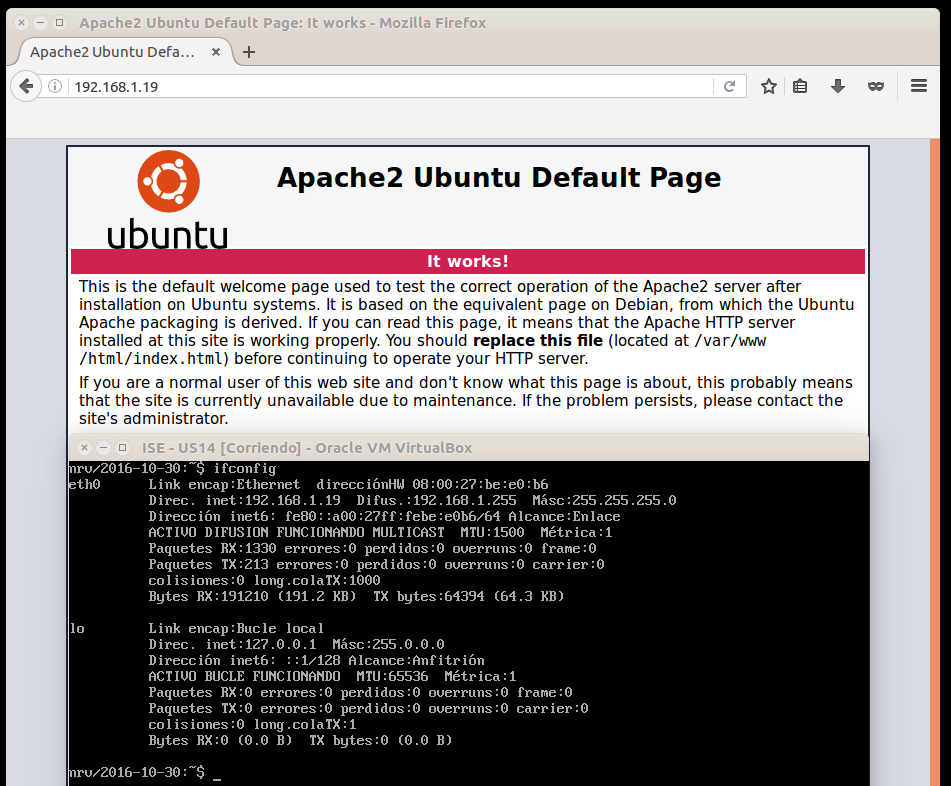
\includegraphics[width=\linewidth]{./Imagenes/9-web-ubuntu.png}
		\vspace{-0.5cm}
		\caption[Servidor web en funcionamiento (máquinas conectadas en modo \textit{bridge}).]{Servidor web en funcionamiento (máquinas conectadas en modo \textit{bridge}).}
		\label{9-web-ubuntu}
	\end{figure}
	
	Para ver si la instalación de php ha funcionado correctamente, he creado un archivos en \textit{/var/www/html} y he accedido desde mi máquina anfitriona, como se puede ver en la figura \ref{9-php-ubuntuserver}. \footnote{Para poder acceder desde la máquina anfitriona a Ubuntu Server he tenido que levantar la interfaz de red \textit{eth1}, para ello he ejecutado el comando \textit{sudo ifconfig eth1} seguido de \textit{sudo dhclient}. Doy por hecho que de aquí en adelante cada vez que necesite acceder a Ubuntu Server desde mi máquina anfitriona estos dos comandos han sido ejecutados previamente.}
	
	\begin{figure}[H]
		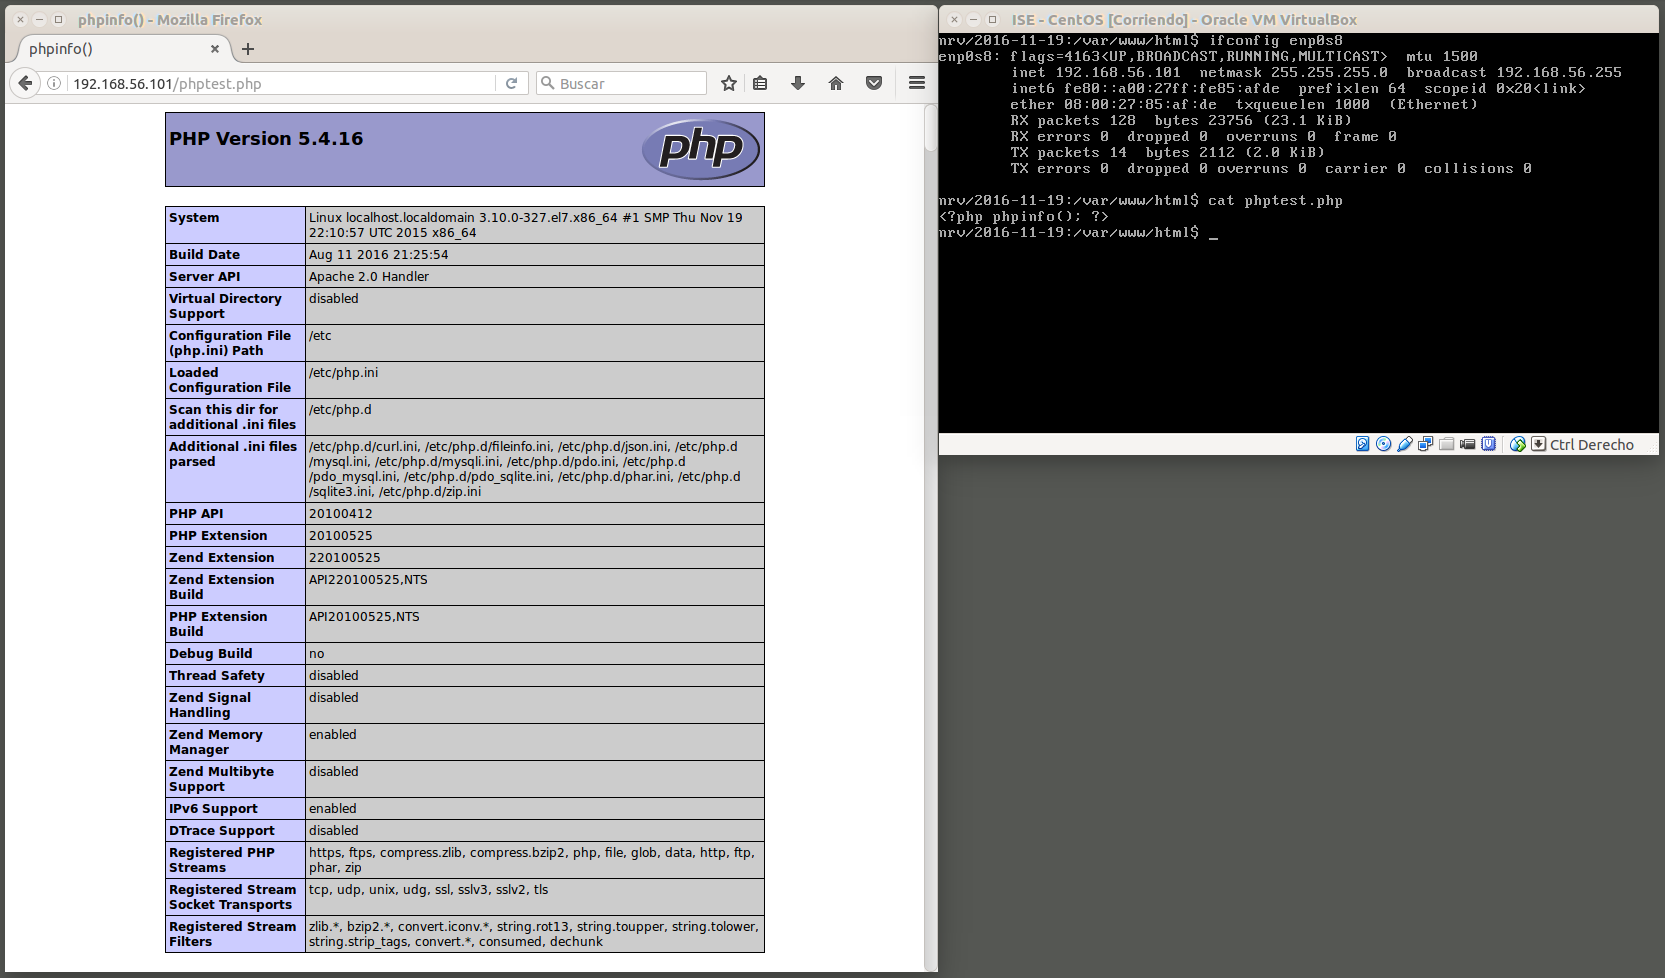
\includegraphics[width=\linewidth]{./Imagenes/9-php-ubuntuserver.png}
		\vspace{-0.5cm}
		\caption[php en funcionamiento (máquinas conectadas en modo \textit{host-only}).]{php en funcionamiento (máquinas conectadas en modo \textit{host-only}).}
		\label{9-php-ubuntuserver}
	\end{figure}
	
	Para ver si la instalación de MySQL ha funcionado correctamente, debemos ejecutar el comando \textit{mysql -u root -p} e introducir la contraseña que se uso para la instalación. Una vez hecho esto, se accede a la consola de MySQl, como se puede ver en la figura \ref{9-mysql-ubuntuserver}.
		
	\begin{figure}[H]
		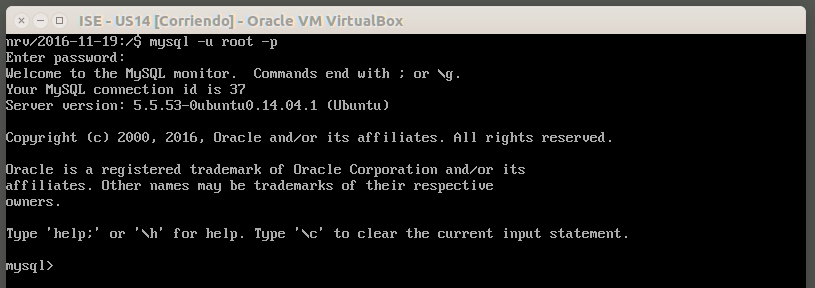
\includegraphics[width=\linewidth]{./Imagenes/9-mysql-ubuntuserver.png}
		\vspace{-0.5cm}
		\caption[mysql en funcionamiento (máquinas conectadas en modo \textit{host-only}).]{mysql en funcionamiento (máquinas conectadas en modo \textit{host-only}).}
		\label{9-mysql-ubuntuserver}
	\end{figure}
	
	A continuación vamos a realizar la instalación en CentOS de Apache + MySQL + Python. Los pasos a seguir son \cite{webcentos}:
	\begin{enumerate}
		\item Instalamos Apache ejecutando: \textit{sudo yum install httpd} \\ Una vez instalado Apache, debemos arrancar el servidor. Para ello ejecutamos: \textit{sudo systemctl start httpd.service}
		\item Instalamos MySQL (MariaDB \footnote{MariaDB es un reemplazo de MySQL.}) con: \textit{sudo yum install mariadb-server mariadb} \\ Una vez instalado MariaDB, debemos arrancar el servidor. Para ello ejecutamos: \textit{sudo systemctl start mariadb}
		\item Instalamos PHP ejecutando: \textit{sudo yum install php php-mysql} \\ Una vez instalado PHP, debemos arrancar el servidor. Para ello ejecutamos: \textit{sudo systemctl start httpd.service}
	\end{enumerate}
	
	Para ver si la instalación de Apache ha funcionado correctamente, desde la máquina anfitriona debemos acceder desde un navegador a la dirección IP de nuestro servidor. En la figura \ref{9-web-centos} podemos ver que la dirección IP es \textit{192.168.1.21} y que funciona correctamente, ya que podemos acceder desde un navegador en la máquina anfitrión. \footnote{Para que funcione correctamente he tenido que habilitar el puerto 80 y el 8080 con \textit{firewall-cmd}.}
		
	\begin{figure}[H]
		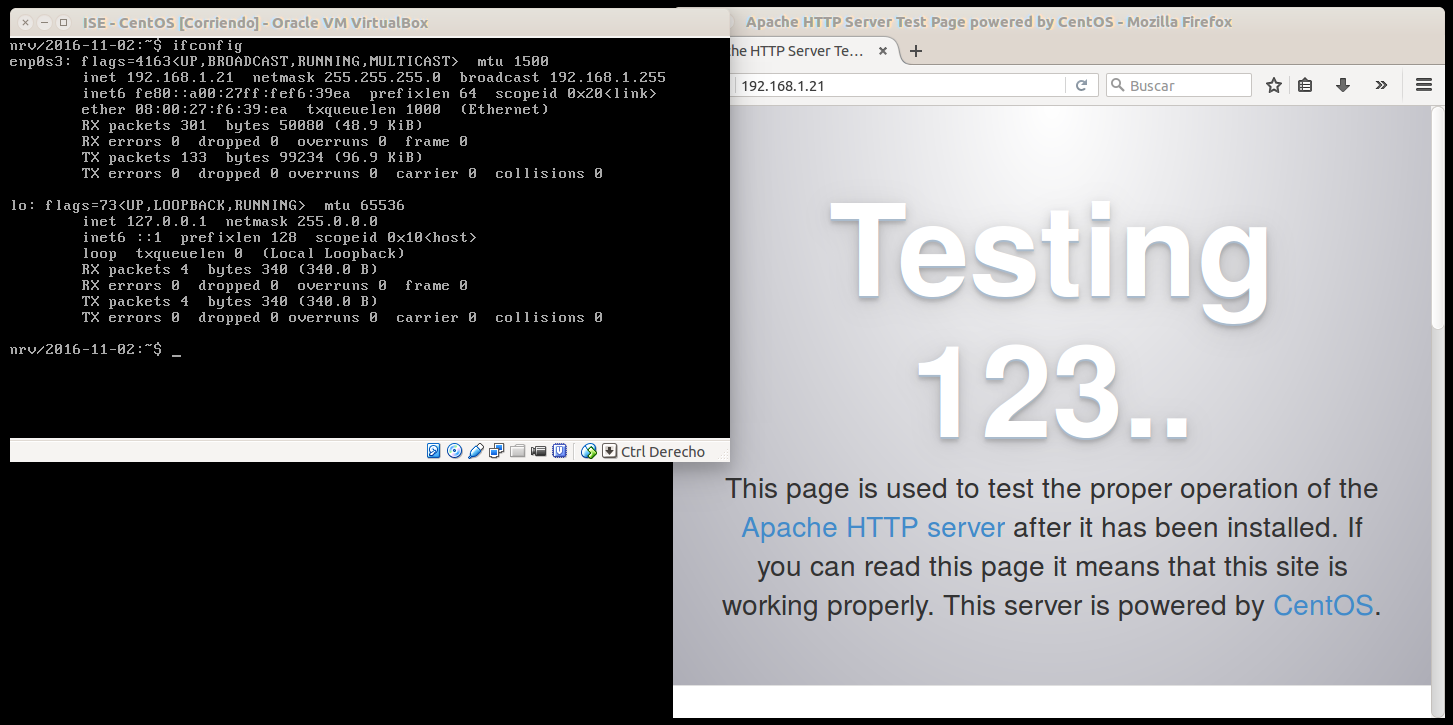
\includegraphics[width=\linewidth]{./Imagenes/9-web-centos.png}
		\vspace{-0.5cm}
		\caption[Servidor web en funcionamiento (CentOS) (máquinas conectadas en modo \textit{bridge}).]{Servidor web en funcionamiento (CentOS) (máquinas conectadas en modo \textit{bridge}).}
		\label{9-web-centos}
	\end{figure}
	
	Para ver si la instalación de php ha funcionado correctamente, he creado un archivos en \textit{/var/www/html} y he accedido desde mi máquina anfitriona, como se puede ver en la figura \ref{9-php-centos}.
		
	\begin{figure}[H]
		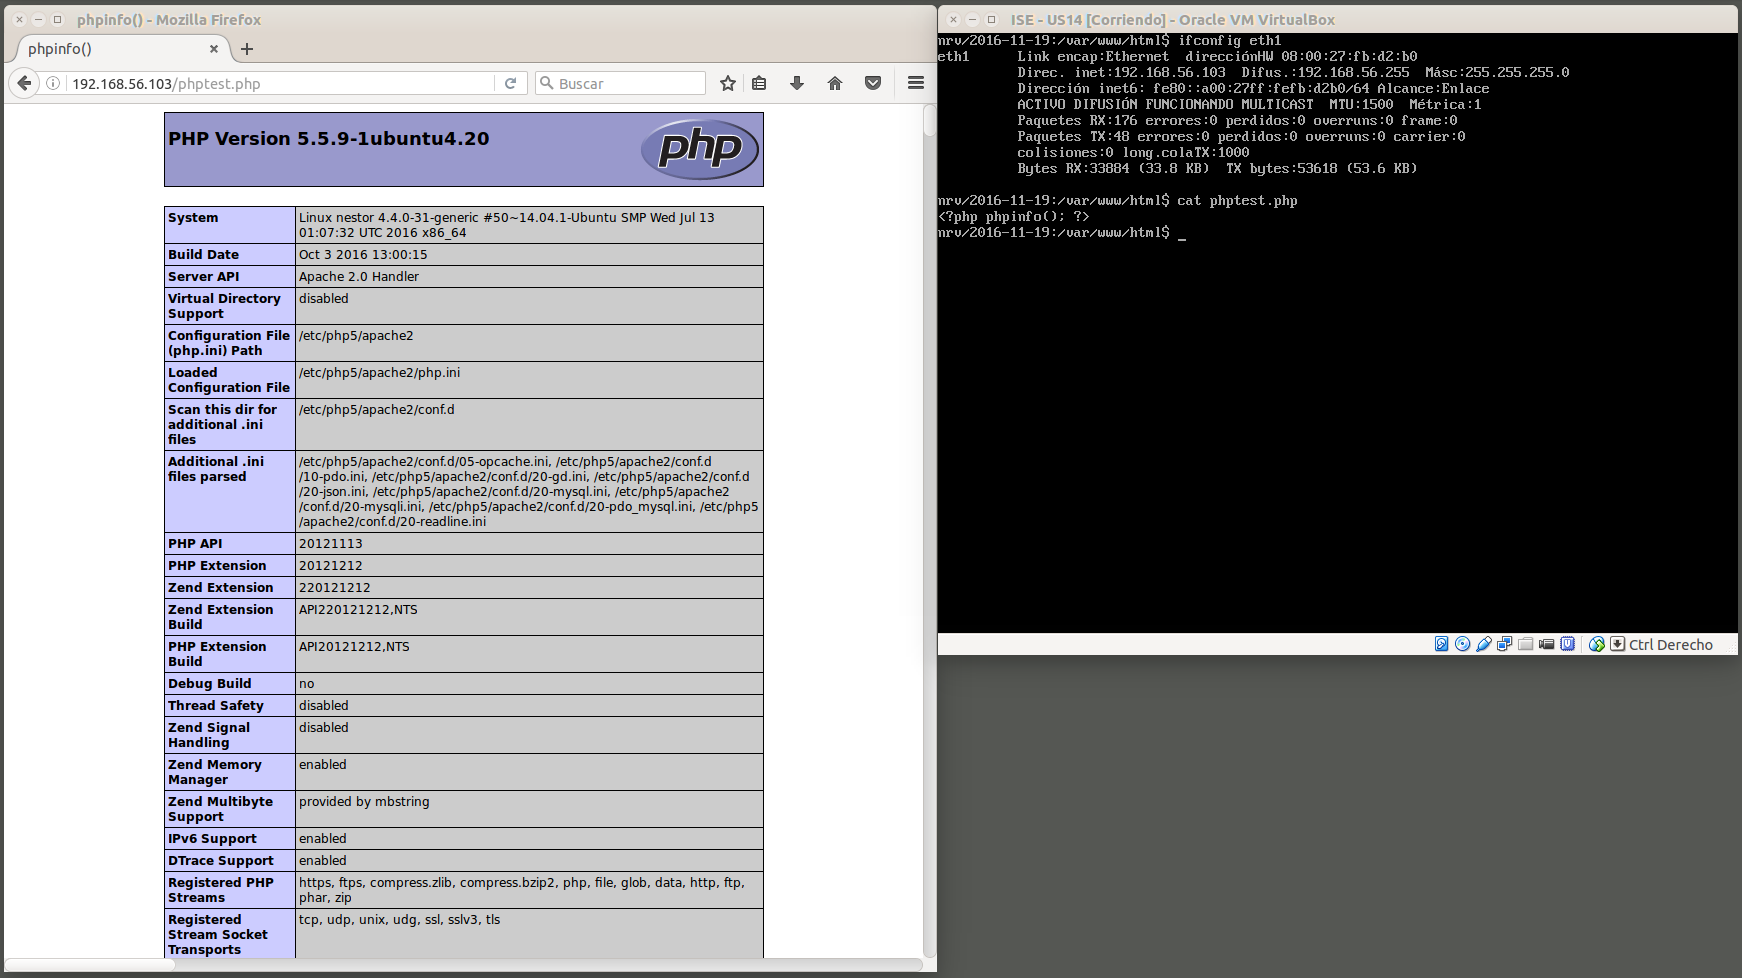
\includegraphics[width=\linewidth]{./Imagenes/9-php-centos.png}
		\vspace{-0.5cm}
		\caption[php en funcionamiento (máquinas conectadas en modo \textit{host-only}).]{php en funcionamiento (máquinas conectadas en modo \textit{host-only}).}
		\label{9-php-centos}
	\end{figure}
	
	Para ver si la instalación de MySQL ha funcionado correctamente, debemos ejecutar el comando \textit{mysql -u root -p}. Cuando nos pida una contraseña, no introducimos ninguna. Una vez hecho esto, se accede a la consola de MariaDB, que como ya dije antes, es un reemplazo de MySQL, como se puede ver en la figura \ref{9-mysql-centos}.
		
	\begin{figure}[H]
		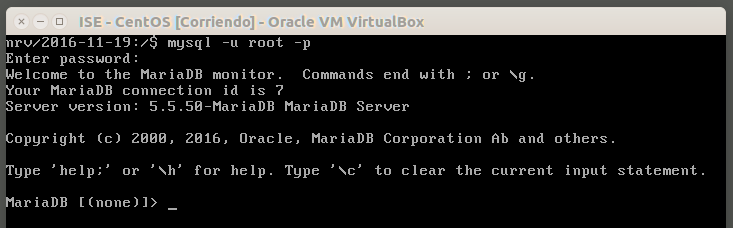
\includegraphics[width=\linewidth]{./Imagenes/9-mysql-centos.png}
		\vspace{-0.5cm}
		\caption[mysql en funcionamiento (máquinas conectadas en modo \textit{host-only}).]{mysql en funcionamiento (máquinas conectadas en modo \textit{host-only}).}
		\label{9-mysql-centos}
	\end{figure}
	
	%%%%%%%%%%%%%%%%%%%%%%%%%%%%%%%%%%%%%%%%%%%%%%%%%%%%
	%%%%%%%%%%%%%%%%%%%% Cuestión 10 %%%%%%%%%%%%%%%%%%%
	%%%%%%%%%%%%%%%%%%%%%%%%%%%%%%%%%%%%%%%%%%%%%%%%%%%%
	\section[Cuestión 10: Realice la instalación usando GUI o PowerShell y compruebe que el servicio está funcionando accediendo a la MV a través de la anfitriona.]{Cuestión 10: Realice la instalación usando GUI o PowerShell y compruebe que el servicio está funcionando accediendo a la MV a través de la anfitriona.}
	
	Para ver si ha funcionado correctamente, desde la máquina anfitriona debemos acceder desde un navegador a la dirección IP de nuestro servidor. En la figura \ref{10-web-windows} podemos ver que la dirección IP es \textit{192.168.1.20} y que funciona correctamente, ya que podemos acceder desde un navegador en la máquina anfitrión.
	
	\begin{figure}[H]
		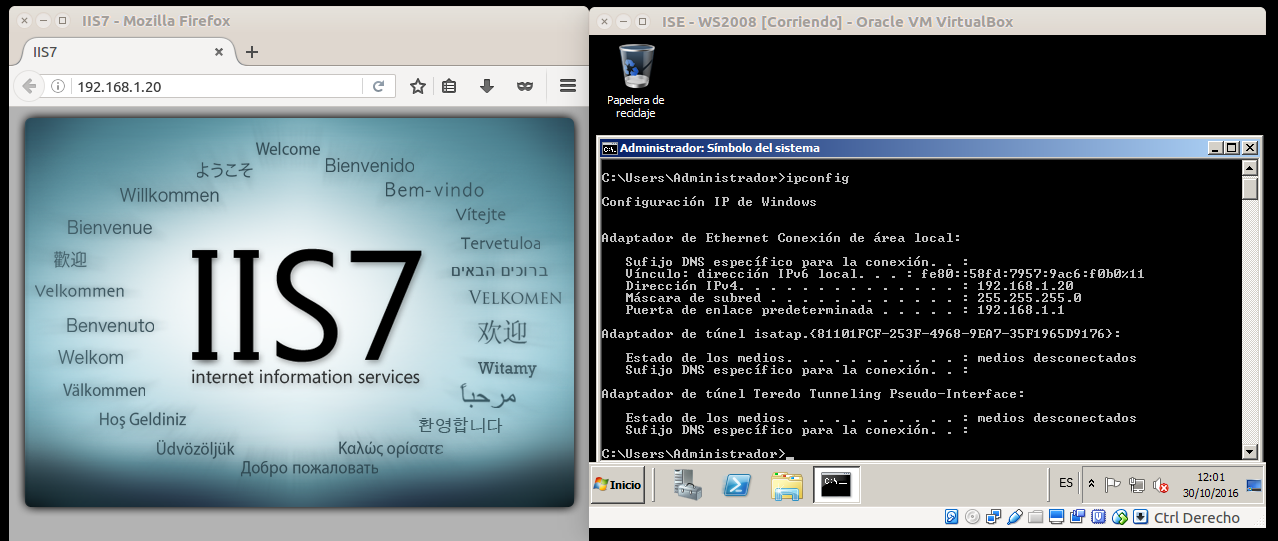
\includegraphics[width=\linewidth]{./Imagenes/10-web-windows.png}
		\vspace{-0.5cm}
		\caption[Servidor web en funcionamiento (Windows Server).]{Servidor web en funcionamiento (Windows Server).}
		\label{10-web-windows}
	\end{figure}
	
	%%%%%%%%%%%%%%%%%%%%%%%%%%%%%%%%%%%%%%%%%%%%%%%%%%%%
	%%%%%%%%%%%%%%%%%%%% Cuestión 11 %%%%%%%%%%%%%%%%%%%
	%%%%%%%%%%%%%%%%%%%%%%%%%%%%%%%%%%%%%%%%%%%%%%%%%%%%
	\section[Cuestión 11: Muestre un ejemplo de uso del comando.]{Cuestión 11: Muestre un ejemplo de uso del comando.}
	
	Como podemos ver en la página de Fedora \cite{patch} un ejemplo de uso del comando sería \textit{patch -p0 -i /tmp/vmware-netfilter.patch} \\
	
	Como podemos ver en las páginas de manual del comando \textit{patch} \cite{manpatch}:
	\begin{itemize}
		\item El argumento \textit{-p0} sirve para dar el nombre del fichero sin modificar.
		\item El argumento \textit{-i} sirve para indicar que debe leer el parche del archivo que tiene a continuación, \textit{/tmp/vmware-nerfilter.patch} en este caso.
	\end{itemize}
	
	Para mostrar como funciona en la práctica, voy a realizar un ejemplo pequeño. Ya que no tengo ningún archivo que parchear ni ningún parche, voy a inventármelos yo.
	\begin{enumerate}
		\item Creamos dos archivos, \textit{version1} y \textit{version2}.
		\item Vemos las diferencias de ambos archivos y creamos el parche a aplicar ejecutando \textit{diff -u version1 version2 > parche.patch}
		\item Parcheamos el archivo \textit{version1} ejecutando \textit{patch -p0 -i parche.patch}
	\end{enumerate}
	
	Todo este proceso se puede ver en la figura \ref{11-patch}.
	\begin{figure}[H]
		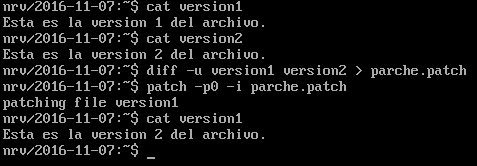
\includegraphics[width=\linewidth]{./Imagenes/11-patch.png}
		\vspace{-0.5cm}
		\caption[Proceso de ``parcheo'' con el comando \textit{patch}.]{Proceso de ``parcheo'' con el comando \textit{patch}.}
		\label{11-patch}
	\end{figure}
	
	%%%%%%%%%%%%%%%%%%%%%%%%%%%%%%%%%%%%%%%%%%%%%%%%%%%%
	%%%%%%%%%%%%%%%%%%%% Cuestión 12 %%%%%%%%%%%%%%%%%%%
	%%%%%%%%%%%%%%%%%%%%%%%%%%%%%%%%%%%%%%%%%%%%%%%%%%%%
	\section[Cuestión 12: Realice la instalación de esta aplicación y pruebe a modificar algún parámetro de algún servicio. Muestre las capturas de pantalla pertinentes así como el proceso de instalación.]{Cuestión 12: Realice la instalación de esta aplicación y pruebe a modificar algún parámetro de algún servicio. Muestre las capturas de pantalla pertinentes así como el proceso de instalación.}
	
	El proceso de instalación lo podemos ver en la página oficial de Webmin \cite{webmin}. Los pasos a seguir son:
	\begin{enumerate}
		\item Editar el archivo \textit{/etc/apt/sources.list} y añadir siguiente línea, cómo podemos ver en la figura \ref{12-1-webmin}.\\
		\textit{deb http://download.webmin.com/download/repository sarge contrib}
		\item Obtenemos la clave GPG con la cual el repositorio está firmado y la instalamos. Para ellos ejecutamos los siguientes comandos en modo \textit{root} como podemos ver en la figura \ref{12-2-webmin}:
		\begin{enumerate}
			\item \textit{cd /root}
			\item \textit{wget http://www.webmin.com/jcameron-key.asc}
			\item \textit{apt-key add jcameron-key.asc}
		\end{enumerate}
		
		\item Actualizamos los repositorios con \textit{sudo apt update} e instalar Webmin con el comando \textit{sudo apt install webmin}, como podemos ver en la figura  \ref{12-3-webmin}.
	\end{enumerate}
	
	\begin{figure}[H]
		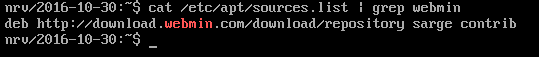
\includegraphics[width=\linewidth]{./Imagenes/12-1-webmin.png}
		\vspace{-0.5cm}
		\caption[Repositorio añadido.]{Repositorio añadido.}
		\label{12-1-webmin}
	\end{figure}
	
	\begin{figure}[H]
		\centering
		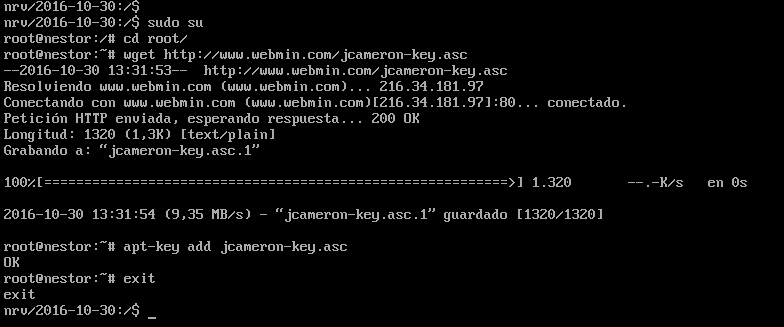
\includegraphics[scale=0.55]{./Imagenes/12-2-webmin.png}
		\caption[Obtención e instalación de la clave GPG.]{Obtención e instalación de la clave GPG.}
		\label{12-2-webmin}
	\end{figure}
	
	\begin{figure}[H]
		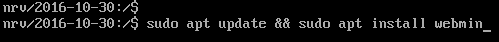
\includegraphics[width=\linewidth]{./Imagenes/12-3-webmin.png}
		\vspace{-0.5cm}
		\caption[Actualizamos los repositorios e instalamos Webmin.]{Actualizamos los repositorios e instalamos Webmin.}
		\label{12-3-webmin}
	\end{figure}
	
	Una vez hemos instalado Webmin, vamos a proceder a cambiar algunos de los parámetros de nuestro servidor. Como podemos ver en las \textit{faq} de Webmin \cite{webminfaq} debemos acceder desde el navegador a la dirección IP de nuestro servidor pero accediendo al puerto 10000. Puede ser que esto nos de problemas, en caso de que sea así, en vez de acceder a mediante \textit{http} debemos acceder mediante \textit{https}. En la figura \ref{12-webmin} podemos ver que la dirección IP de mi servidor es \textit{192.168.1.29}, por lo tanto debemos acceder a través de la dirección \textit{https://192.168.1.29:10000}. Una vez en la página, los datos para acceder son el nombre de usuario de nuestro servidos y la contraseña del mismo.
	
	\begin{figure}[H]
		\centering
		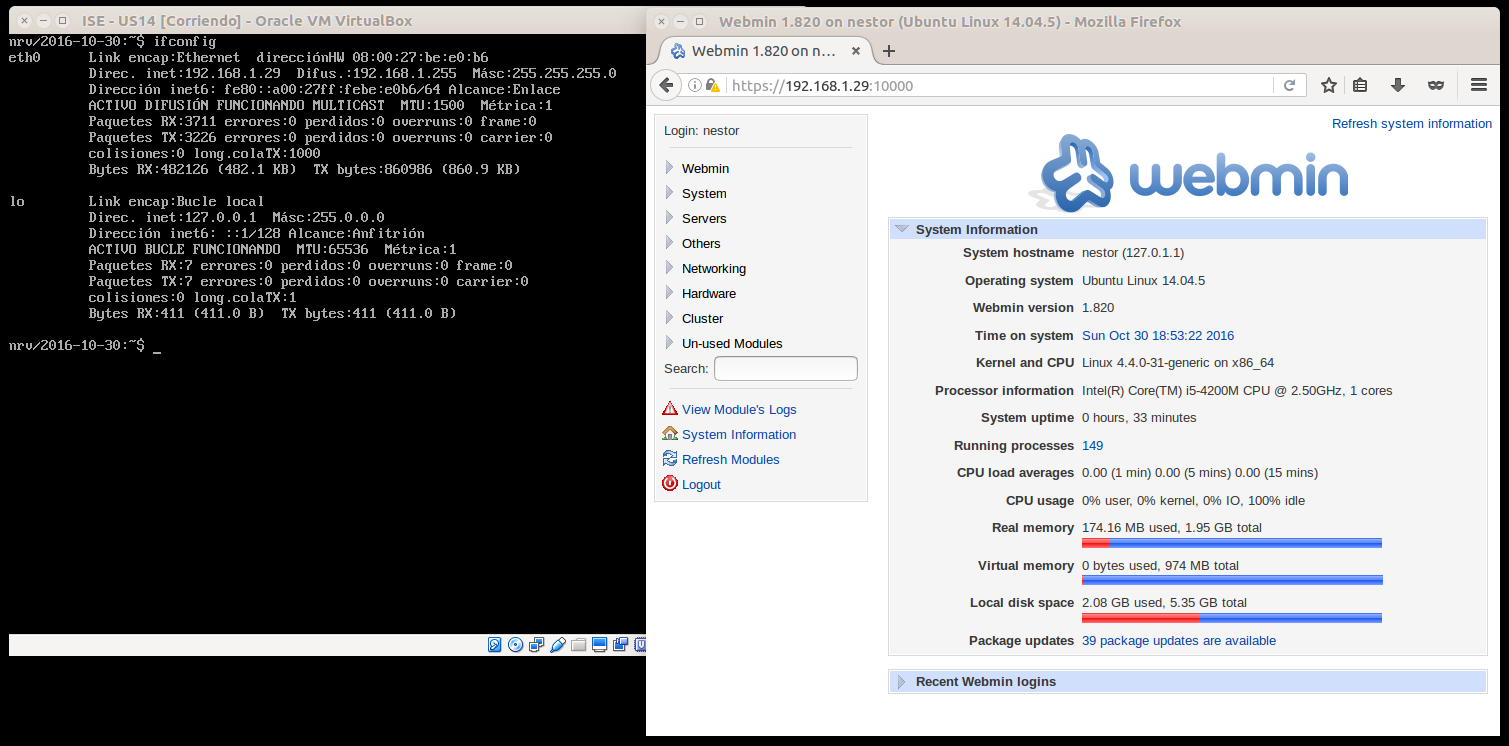
\includegraphics[scale=0.28]{./Imagenes/12-webmin.png}
		\caption[Webmin en funcionamiento (máquinas conectadas en modo \textit{bridge}).]{Webmin en funcionamiento (máquinas conectadas en modo \textit{bridge}).}
		\label{12-webmin}
	\end{figure}
	
	En el menú de la izquierda hay múltiples opciones que nos permiten realizar distintas tareas. Hay dos de ellas que me parecen realmente interesantes. La primera se encuentra dentro del menú \textit{System}, en la sección \textit{Bootup and Shutdown}. Esta sección nos permite manipular los servicios que se están ejecutando en nuestro servidor, permitiéndonos, por ejemplo, parar un servicio, reiniciarlo e incluso elegir si debe iniciarse o no al encender el sistema. Como podemos ver en la figura \ref{12-pararssh}, podría parar mi servidor ssh.
	
	\begin{figure}[H]
		\centering
		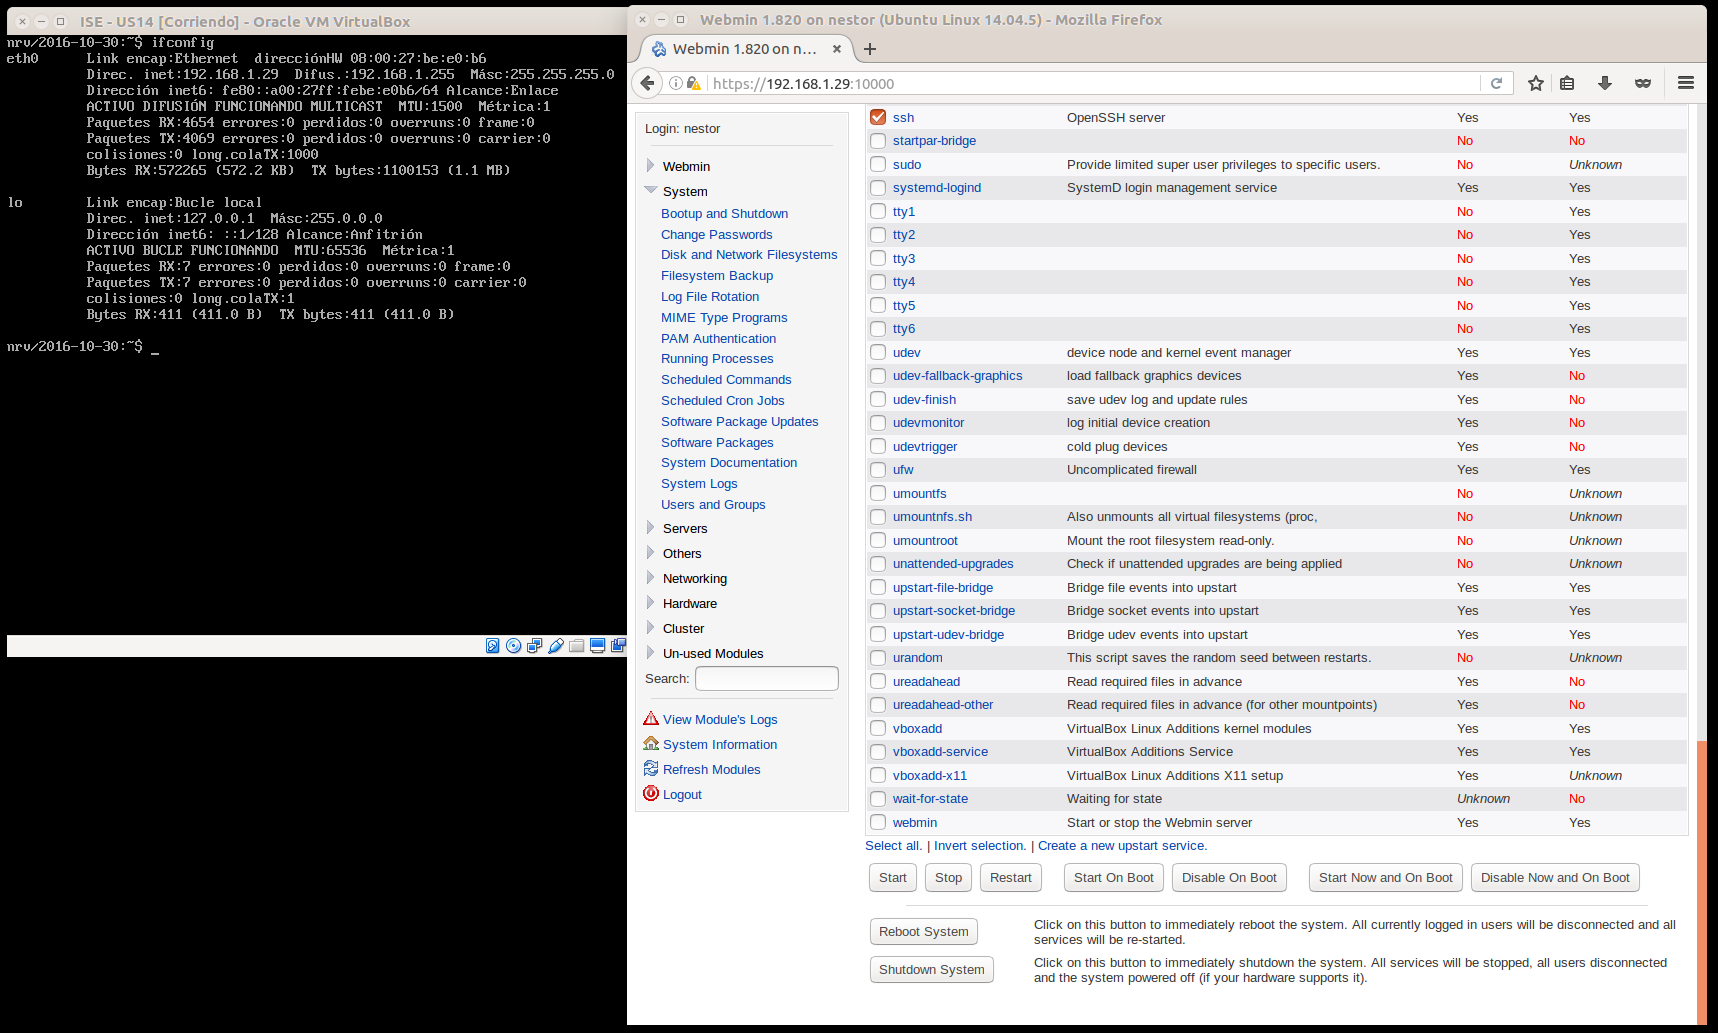
\includegraphics[scale=0.23]{./Imagenes/12-pararssh.png}
		\caption[Manipulación de servicios con Webmin (máquinas conectadas en modo \textit{bridge}).]{Manipulación de servicios con Webmin (máquinas conectadas en modo \textit{bridge}).}
		\label{12-pararssh}
	\end{figure}
	
	La segunda característica se encuentra dentro del menú \textit{Others}, en la sección \textit{Command Shell}. Esta sección nos permite ejecutar comandos en nuestro servidor desde Webmin como podemos ver en la figura \footnote{La dirección IP de mi servidor ha cambiado, ahora es \textit{192.168.1.30} como se puede ver en la figura.} \ref{12-comandos}.
	
	\begin{figure}[H]
		\centering
		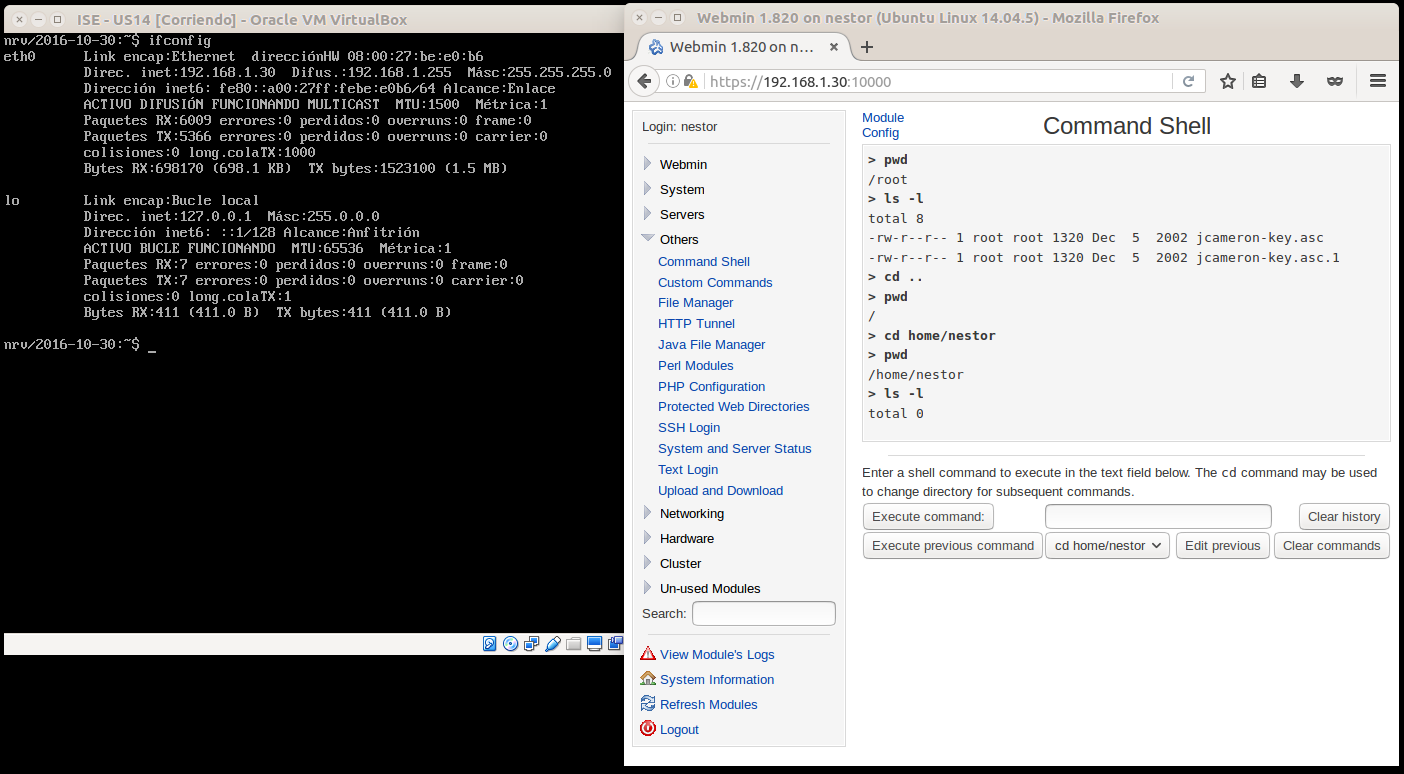
\includegraphics[scale=0.28]{./Imagenes/12-comandos.png}
		\caption[Ejecución de comandos mediante Webmin (máquinas conectadas en modo \textit{bridge}).]{Ejecución de comandos mediante Webmin (máquinas conectadas en modo \textit{bridge}).}
		\label{12-comandos}
	\end{figure}
	
	%%%%%%%%%%%%%%%%%%%%%%%%%%%%%%%%%%%%%%%%%%%%%%%%%%%%
	%%%%%%%%%%%%%%%%%%%% Cuestión 13 %%%%%%%%%%%%%%%%%%%
	%%%%%%%%%%%%%%%%%%%%%%%%%%%%%%%%%%%%%%%%%%%%%%%%%%%%
	\section[Cuestión 13 : Instale phpMyAdmin, indique cómo lo ha realizado y muestre algunas capturas de pantalla. Configure PHP para poder importar BDs de hasta 25MiB (en vez de los 8 MiB de límite por defecto). Indique cómo ha realizado el proceso y muestre capturas de pantalla.]{Cuestión 13 : Instale phpMyAdmin, indique cómo lo ha realizado y muestre algunas capturas de pantalla. Configure PHP para poder importar BDs de hasta 25MiB (en vez de los 8 MiB de límite por defecto). Indique cómo ha realizado el proceso y muestre capturas de pantalla.}
	
	Para instalar phpMyAdmin vamos a seguir los pasos que podemos ver en la página de Ubuntu, tanto en la documentación oficial \cite{phpmyadminubuntu} como en la Wiki de la comunidad \cite{phpmyadminubuntuwiki}:
	\begin{enumerate}
		\item Primero instalamos phpMyAdmin con el comando \textit{sudo apt install phpmyadmin}. Cuando nos pregunte que servidor web vamos a usar, elegimos \textit{apache2}.
		\item Ahora tenemos que modificar el archivo \textit{/etc/apache2/apache2.conf} y añadir la línea \textit{Include /etc/phpmyadmin/apache.conf}. El resultado lo podemos ver en la figura \ref{13-phpmyadmin}.
		\item Ahora podemos acceder desde nuestra máquina anfitriona escribiendo en el navegador la dirección IP de nuestro servidor seguido de \textit{/phpmyadmin}. En mi caso, la dirección IP es \textit{192.168.1.31} así que para entrar debemos escribir en la barra del navegador \textit{http://192.168.1.32/phpmyadmin}. Podemos entrar perfectamente, como vemos en la figura \ref{13-phpmyadminfuncionando}. Una vez en la página, el nombre de usuario para acceder es \textit{root} y la contraseña es la de nuestro servidor.
	\end{enumerate}
	
	\begin{figure}[H]
		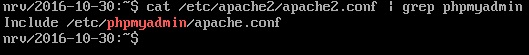
\includegraphics[width=\linewidth]{./Imagenes/13-includephpmyadmin.png}
		\vspace{-0.5cm}
		\caption[Archivo modificado.]{Archivo modificado.}
		\label{13-phpmyadmin}
	\end{figure}
	
	\begin{figure}[H]
		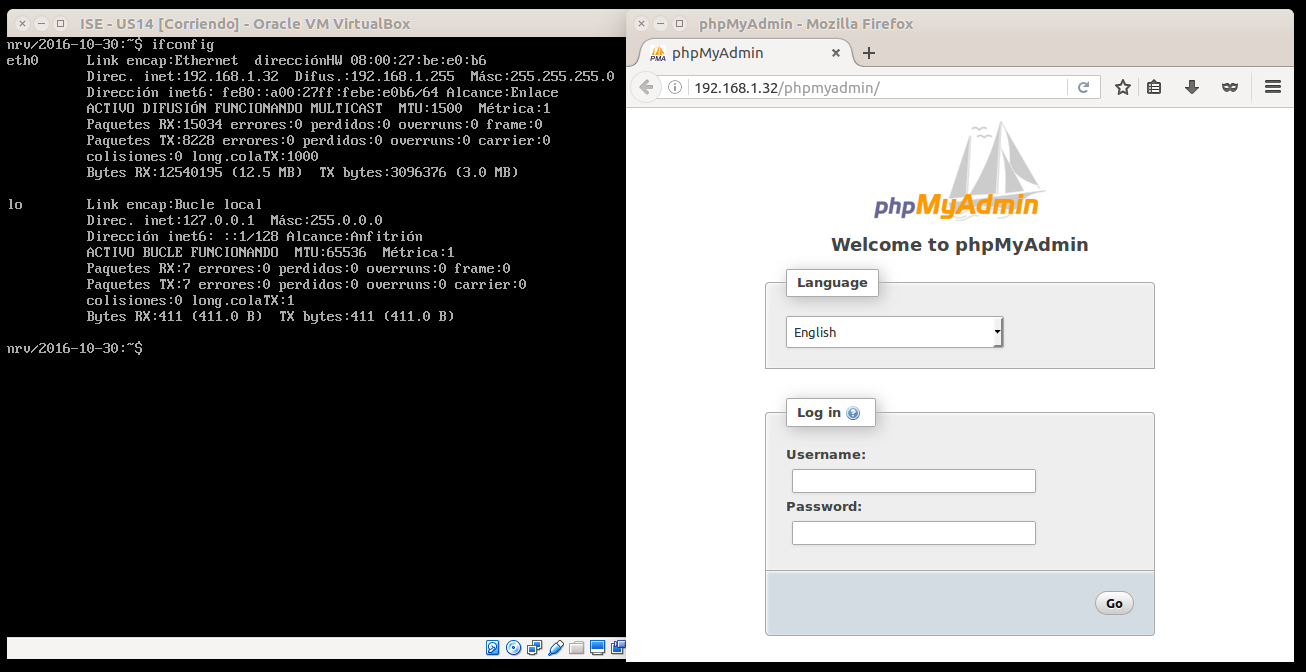
\includegraphics[width=\linewidth]{./Imagenes/13-phpmyadminfuncionando.png}
		\vspace{-0.5cm}
		\caption[phpMyAdmin funcionando (máquinas conectadas en modo \textit{bridge}).]{phpMyAdmin funcionando (máquinas conectadas en modo \textit{bridge}).}
		\label{13-phpmyadminfuncionando}
	\end{figure}
	
	El proceso para cambiar el tamaño máximo de las bases de datos lo podemos ver en la página de phpMyAdmin \cite{phpmyadfilesize}. Tenemos que modificar el archivo \textit{/etc/php5/apache2/php.ini}:
	\begin{itemize}
		\item Debemos cambiar el valor de \textit{upload\_max\_filesize}. El valor que trae por defecto es de 2M, nosotros lo cambiamos por 25M como podemos ver en la figura \ref{13-upload_max_filesize}.
		\item Debemos cambiar el valor de \textit{post\_max\_size}. El valor que trae por defecto es de 8M, nosotros lo cambiamos a 25M como podemos ver en la figura \ref{13-post_max_size}.
	\end{itemize}
	
	\begin{figure}[H]
		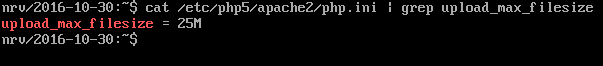
\includegraphics[width=\linewidth]{./Imagenes/13-upload_max_filesize.png}
		\vspace{-0.5cm}
		\caption[upload\_max\_filesize con el nuevo valor.]{upload\_max\_filesize con el nuevo valor.}
		\label{13-upload_max_filesize}
	\end{figure}
	
	\begin{figure}[H]
		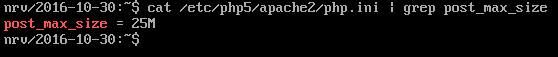
\includegraphics[width=\linewidth]{./Imagenes/13-post_max_size.png}
		\vspace{-0.5cm}
		\caption[post\_max\_size con el nuevo valor.]{post\_max\_size con el nuevo valor.}
		\label{13-post_max_size}
	\end{figure}
	
	Una vez hemos aplicado los cambios, debemos reiniciar el servicio apache2 con el comando \textit{sudo service apache2 restart}. Si ahora nos dirigimos a \textit{phpMyAdmin} desde el navegador e intentamos subir una archivo, podemos ver que el tamaño máximo permitido es 25MiB, tal y cómo se ve en la figura \ref{13-tamanio25}.
	
	\begin{figure}[H]
		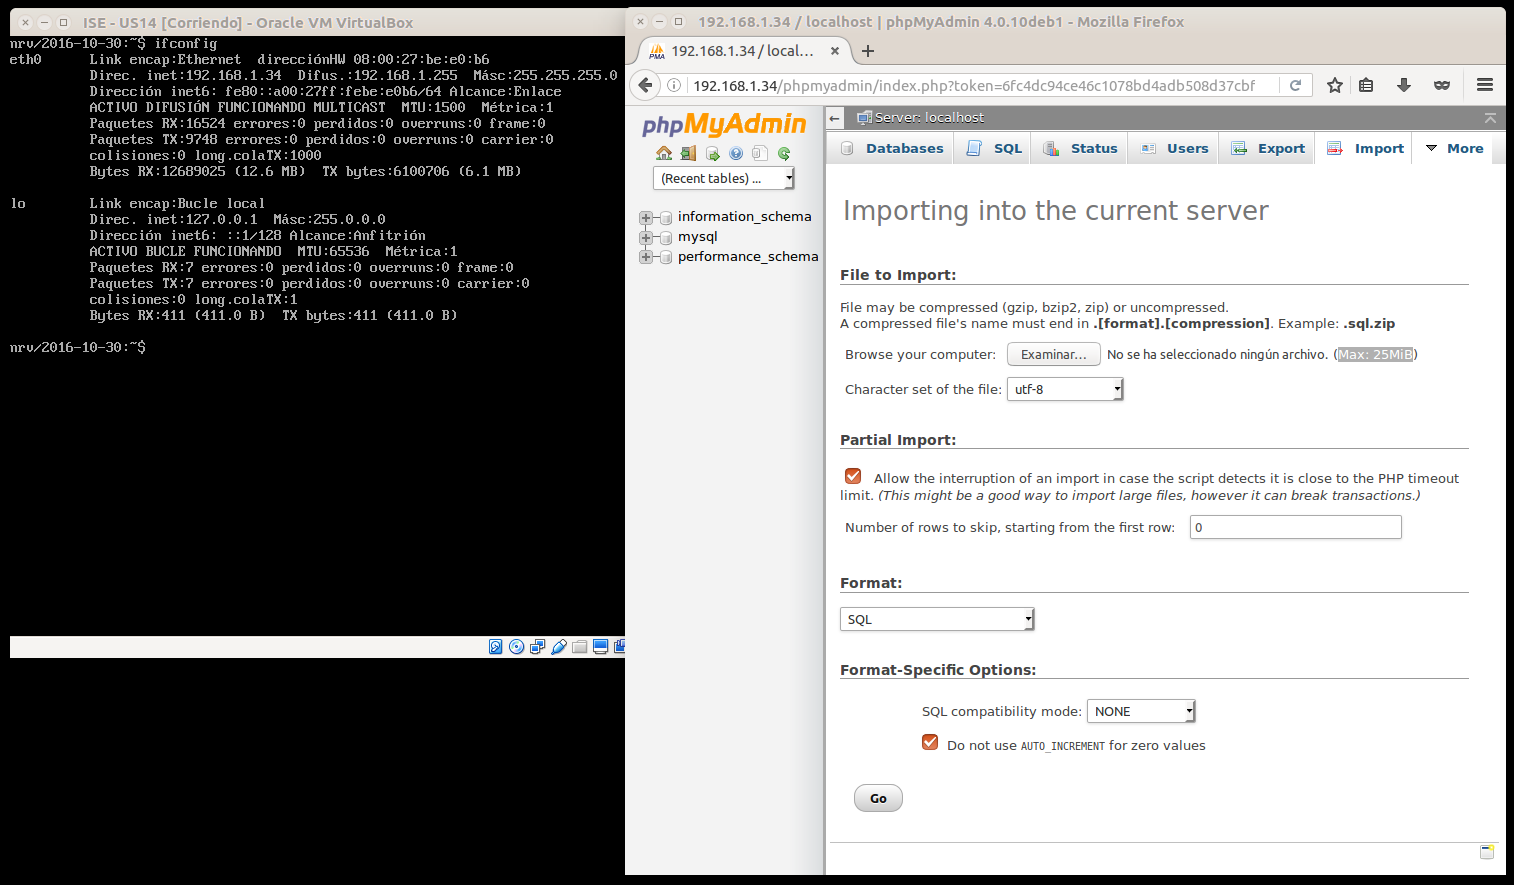
\includegraphics[width=\linewidth]{./Imagenes/13-tamanio25.png}
		\vspace{-0.5cm}
		\caption[El tamaño máximo permitido es 25MiB (máquinas conectadas en modo \textit{bridge}).]{El tamaño máximo permitido es 25MiB (máquinas conectadas en modo \textit{bridge}).}
		\label{13-tamanio25}
	\end{figure}
	
	%%%%%%%%%%%%%%%%%%%%%%%%%%%%%%%%%%%%%%%%%%%%%%%%%%%%
	%%%%%%%%%%%%%%%%%%%% Cuestión 14 %%%%%%%%%%%%%%%%%%%
	%%%%%%%%%%%%%%%%%%%%%%%%%%%%%%%%%%%%%%%%%%%%%%%%%%%%
	\section[Cuestión 14: Viste al menos una de las webs de los software mencionados y pruebe las demos que ofrecen realizando capturas de pantalla y comentando qué está realizando.]{Cuestión 14: Viste al menos una de las webs de los software mencionados y pruebe las demos que ofrecen realizando capturas de pantalla y comentando qué está realizando.}
	
	Yo voy a probar Parallels Plesk \cite{parallelplesk}. En la página de Parallels Plesk podemos probar una demo para ver las opciones que tiene. Lo primero que vemos al acceder es lo que se muestra en la figura \ref{14-inicio}.
	
	\begin{figure}[H]
		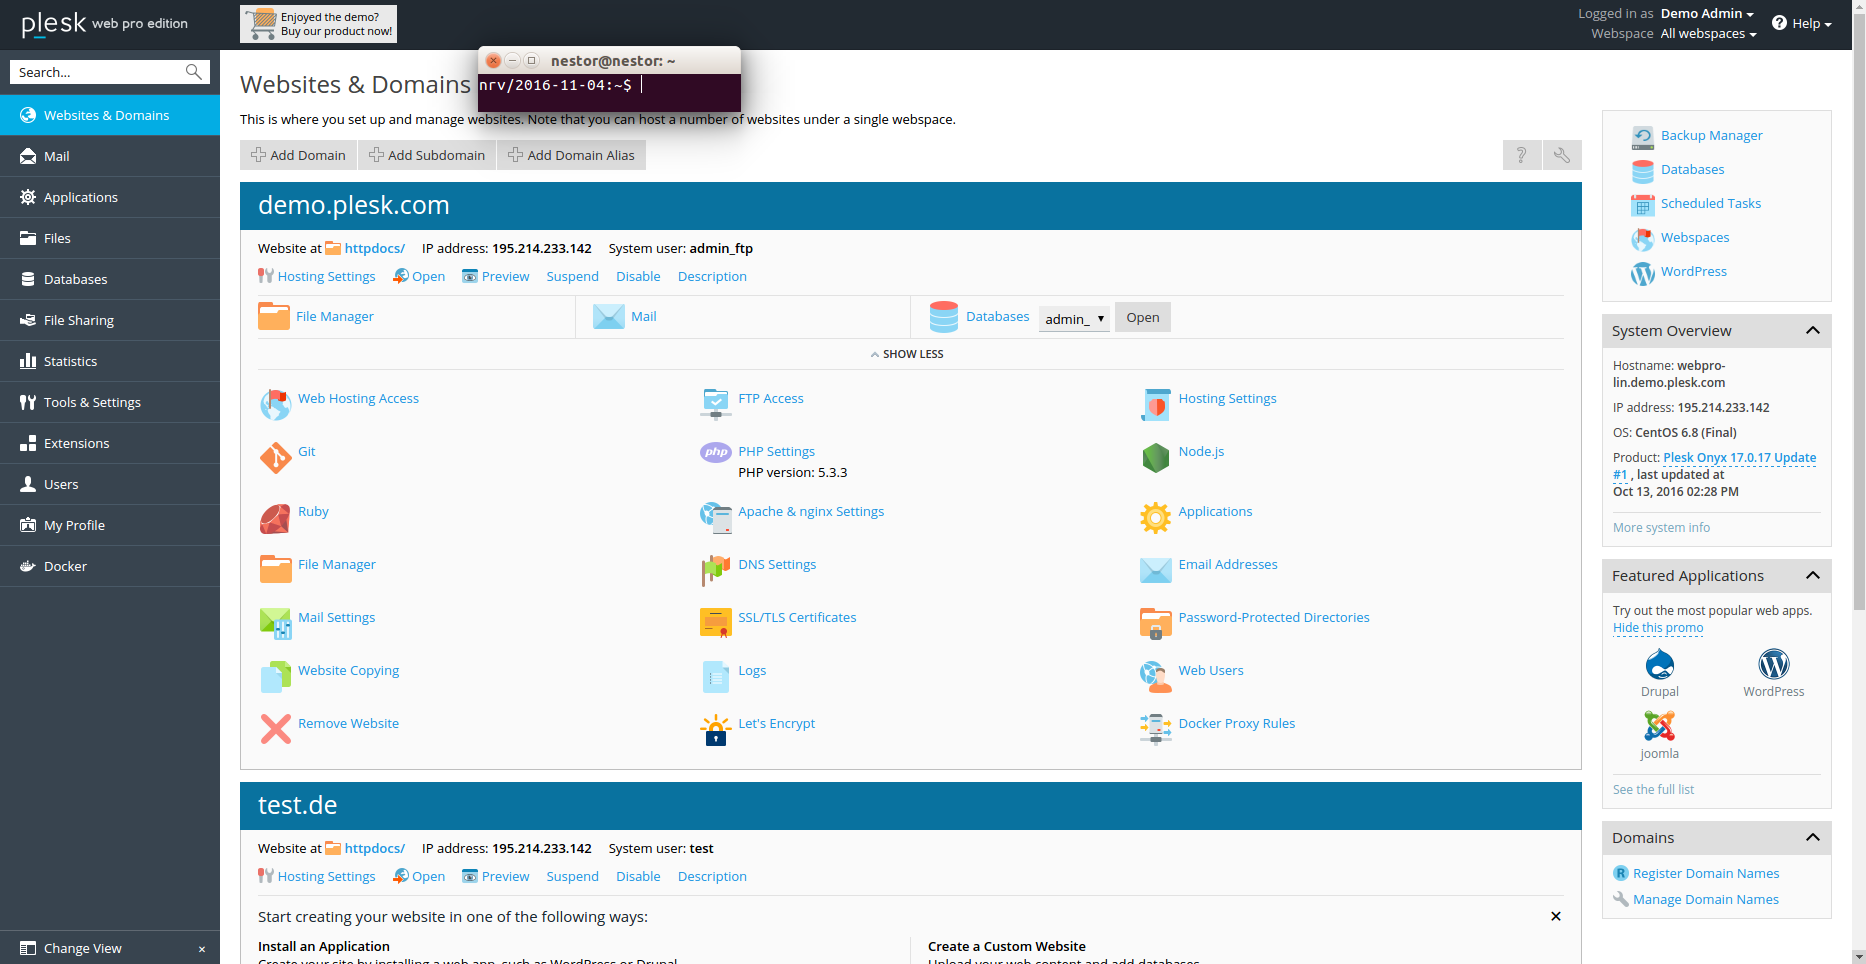
\includegraphics[width=\linewidth]{./Imagenes/14-inicio.png}
		\vspace{-0.5cm}
		\caption[Inicio Parallels Plesk.]{Inicio Parallels Plesk.}
		\label{14-inicio}
	\end{figure}
	
	Cómo podemos ver, se pueden hacer muchas cosas distintas. Las menús más interesantes para mí son \textit{Files}, \textit{Statistics} y \textit{Tools \& Settings}. Veamos cada una de ellas más en profundidad. \\
	
	El menú \textit{Statistics}, como podemos ver en la figura \ref{14-statistics}, nos permite ver estadísticas de nuestro servidor, como puede ser el ancho de banda consumido o el espacio en disco usado.
	\begin{figure}[H]
		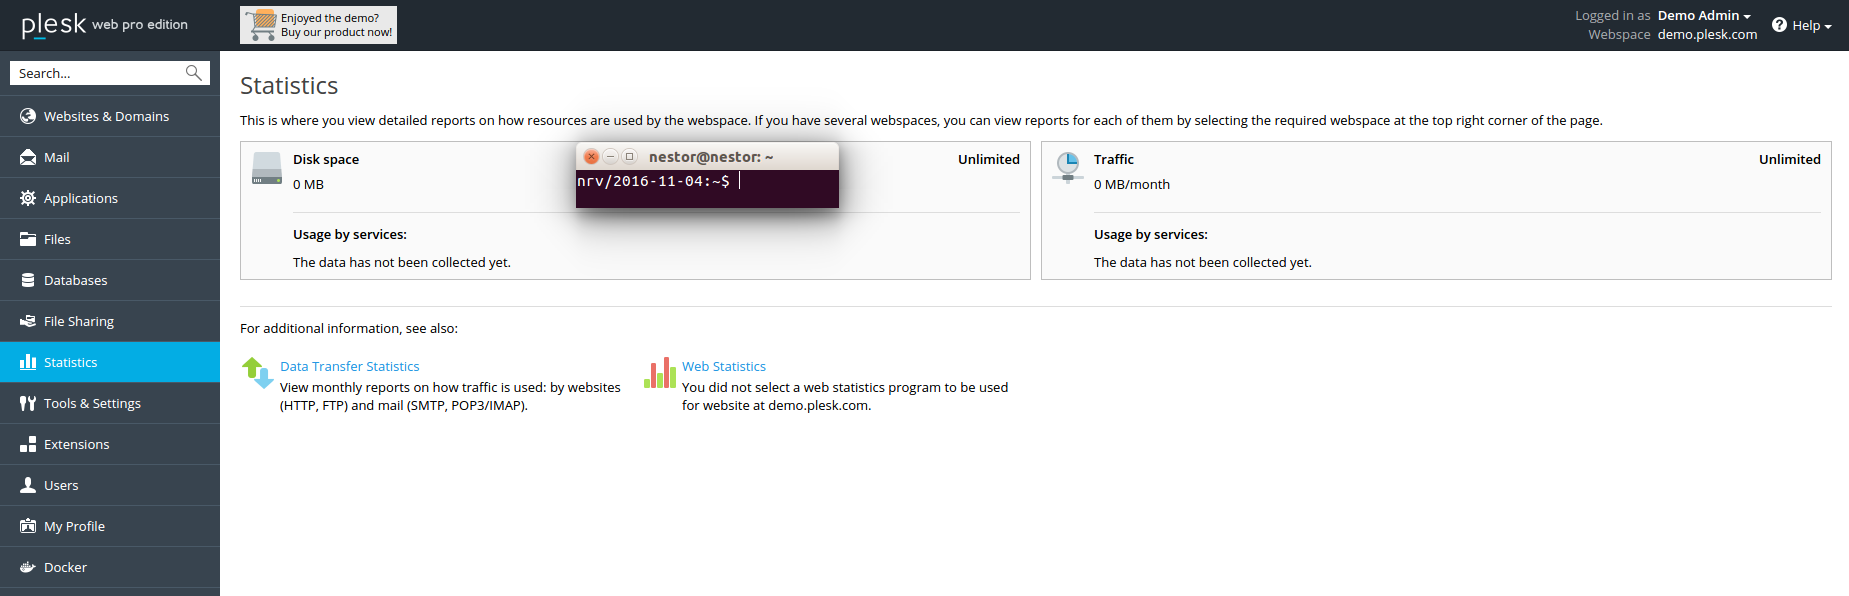
\includegraphics[width=\linewidth]{./Imagenes/14-statistics.png}
		\vspace{-0.5cm}
		\caption[Estadísticas del servidor desde Parallels Plesk.]{Estadísticas del servidor desde Parallels Plesk.}
		\label{14-statistics}
	\end{figure}
	
	El menú \textit{Tools \& Settings}, como podemos ver en la figura \ref{14-tools}, nos permite configurar y usar distintas opciones para nuestro servidor, como podría ser adquirir un certificado SSL, activar un filtro de Spam para el correo y obtener información del servidor.
	\begin{figure}[H]
		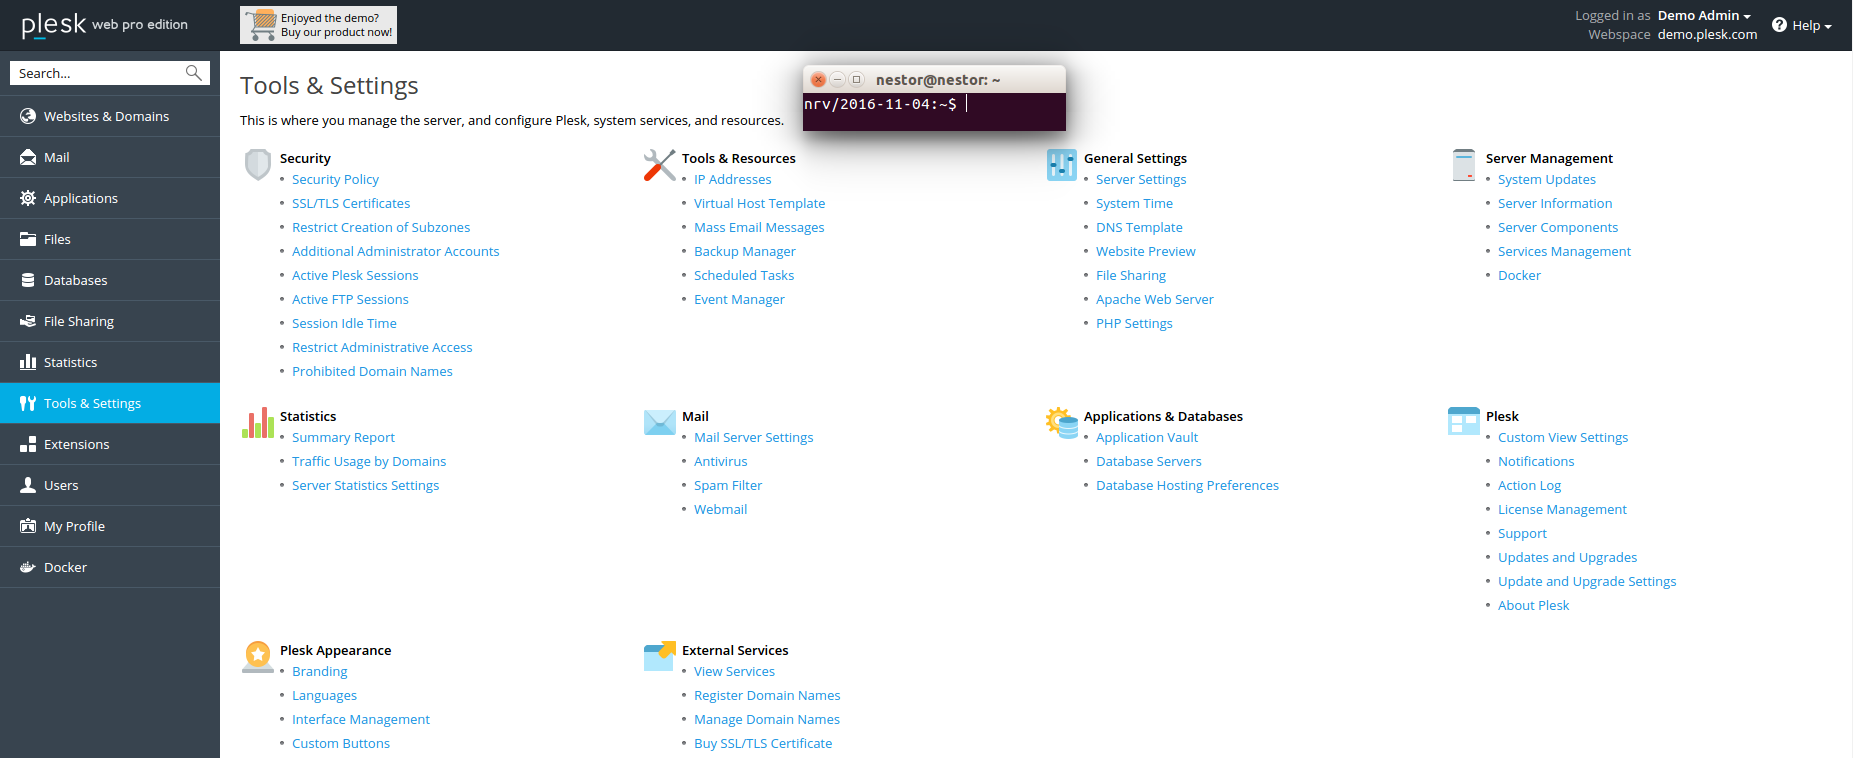
\includegraphics[width=\linewidth]{./Imagenes/14-tools.png}
		\vspace{-0.5cm}
		\caption[Ajustes y herramientas del servidor desde Parallels Plesk.]{Ajustes y herramientas  del servidor desde Parallels Plesk.}
		\label{14-tools}
	\end{figure}
	
	%%%%%%%%%%%%%%%%%%%%%%%%%%%%%%%%%%%%%%%%%%%%%%%%%%%%
	%%%%%%%%%%%%%%%%%%%% Cuestión 15 %%%%%%%%%%%%%%%%%%%
	%%%%%%%%%%%%%%%%%%%%%%%%%%%%%%%%%%%%%%%%%%%%%%%%%%%%
	\section[Cuestión 15:]{Cuestión 15:}
	
	\subsection[a) Ejecute los ejemplos de find, grep.]{a) Ejecute los ejemplos de find, grep.}
	
	\begin{figure}[H]
		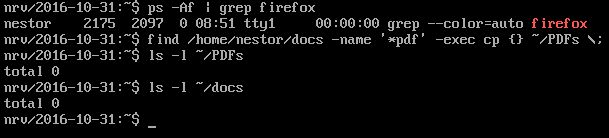
\includegraphics[width=\linewidth]{./Imagenes/15-grepfind.png}
		\vspace{-0.5cm}
		\caption[Ejecución de grep y find.]{Ejecución de grep y find.}
		\label{15-grepfind}
	\end{figure}
	
	La ejecución del comando \textit{find} no proporciona ningún resultado, porque como podemos ver en la figura \ref{15-grepfind} no había ningún pdf en \textit{/home/nestor/docs}.
	
	\subsection[b) Escriba el script que haga uso de sed para cambiar la configuración de ssh y reiniciar el servicio.]{b) Escriba el script que haga uso de sed para cambiar la configuración de ssh y reiniciar el servicio.}
	
	Para ver el funcionamiento de \textit{sed} podemos visitar las páginas de manual del comando \cite{mansed}. Una vez sabemos como funciona, el resultado lo podemos ver en el script \footnote{El script se encuentra dentro de la carpeta \textit{Archivos auxiliares}.} \ref{scriptsed}. \\
	
	\lstset{language=bash, xleftmargin=-1cm, basicstyle=\footnotesize}	
	\begin{lstlisting}[label={scriptsed}]
	#!/bin/bash/
	sed -i `s/.*PasswordAuthentication no.*/PasswordAuthentication yes/'
	    /etc/ssh/sshd_config
	service ssh restart
	sleep 180
	sed -i `s/.*PasswordAuthentication yes.*/PasswordAuthentication no/'
	    /etc/ssh/sshd_config
	service ssh restart
	\end{lstlisting}
	
	\subsection[c) Muestre un ejemplo de uso para awk.]{c) Muestre un ejemplo de uso para awk.}
	
	\begin{figure}[H]
		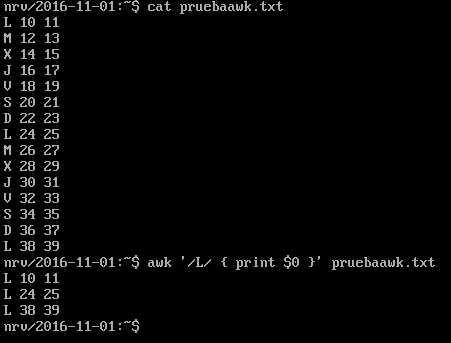
\includegraphics[width=\linewidth]{./Imagenes/15-awk.png}
		\vspace{-0.5cm}
		\caption[Ejecución de awk.]{Ejecución de awk.}
		\label{15-awk}
	\end{figure}
	
	Con este comando hemos conseguido mostrar por pantalla sólo las líneas correspondientes a los lunes, es decir, los que empiezan por \textit{L}.
	
	%%%%%%%%%%%%%%%%%%%%%%%%%%%%%%%%%%%%%%%%%%%%%%%%%%%%
	%%%%%%%%%%%%%%%%%%%% Cuestión 16 %%%%%%%%%%%%%%%%%%%
	%%%%%%%%%%%%%%%%%%%%%%%%%%%%%%%%%%%%%%%%%%%%%%%%%%%%
	\section[Cuestión 16: Escriba el script para cambiar el acceso a ssh usando PHP o Python.]{Cuestión 16: Escriba el script para cambiar el acceso a ssh usando PHP o Python.}
	
	El resultado obtenido lo podemos ver en el script \footnote{El script se encuentra dentro de la carpeta \textit{Archivos auxiliares}.} \ref{scriptpython}.
	
	\lstset{language=python, xleftmargin=-1cm, breaklines=true, basicstyle=\footnotesize}	
	\begin{lstlisting}[label={scriptpython}]
	#!/usr/bin/python
	import subprocess
	subprocess.call([``sudo sed -i 's/.*PasswordAuthentication no.*/PasswordAuthentication yes/' sshd_config''], shell=True)
	subprocess.call([``sudo service ssh restart''], shell=True)
	subprocess.call([``sleep 180''], shell=True)
	subprocess.call([``sudo sed -i 's/.*PasswordAuthentication yes.*/PasswordAuthentication no/' sshd_config''], shell=True)
	subprocess.call([``sudo service ssh restart''], shell=True)
	\end{lstlisting}
	
	%%%%%%%%%%%%%%%%%%%%%%%%%%%%%%%%%%%%%%%%%%%%%%%%%%%%
	%%%%%%%%%%%%%%%%%%%% Cuestión 17 %%%%%%%%%%%%%%%%%%%
	%%%%%%%%%%%%%%%%%%%%%%%%%%%%%%%%%%%%%%%%%%%%%%%%%%%%
	\section[Cuestión 17: Abra una consola de Powershell y pruebe a parar un programa en ejecución (p.ej), realice capturas de pantalla y comente lo que muestra.]{Cuestión 17: Abra una consola de Powershell y pruebe a parar un programa en ejecución (p.ej), realice capturas de pantalla y comente lo que muestra.}
	
	Para ver que comandos debo usar, he visitado la página de Microsoft \cite{ps}.
	
	Los pasos para parar un programa en ejecución son: 
	\begin{enumerate}
		\item Con el comando \textit{Get-Process} obtenemos un listado de los procesos en ejecución, como podemos ver en la figura \ref{17-getprocess}.
		\item Con el comando \textit{Stop-Process -Name VBoxService} paramos el proceso VBoxService, como podemos ver en la figura \ref{17-stopprocess}. Nos pedirá una confirmación, así que le decimos que sí estamos seguro.
		\item Podemos comprobar que se ha parado correctamente ejecutando de nuevo el comando \textit{Get-Process}, como podemos ver en la figura \ref{17-getprocess2}
	\end{enumerate}
	
	\begin{figure}[H]
		\centering
		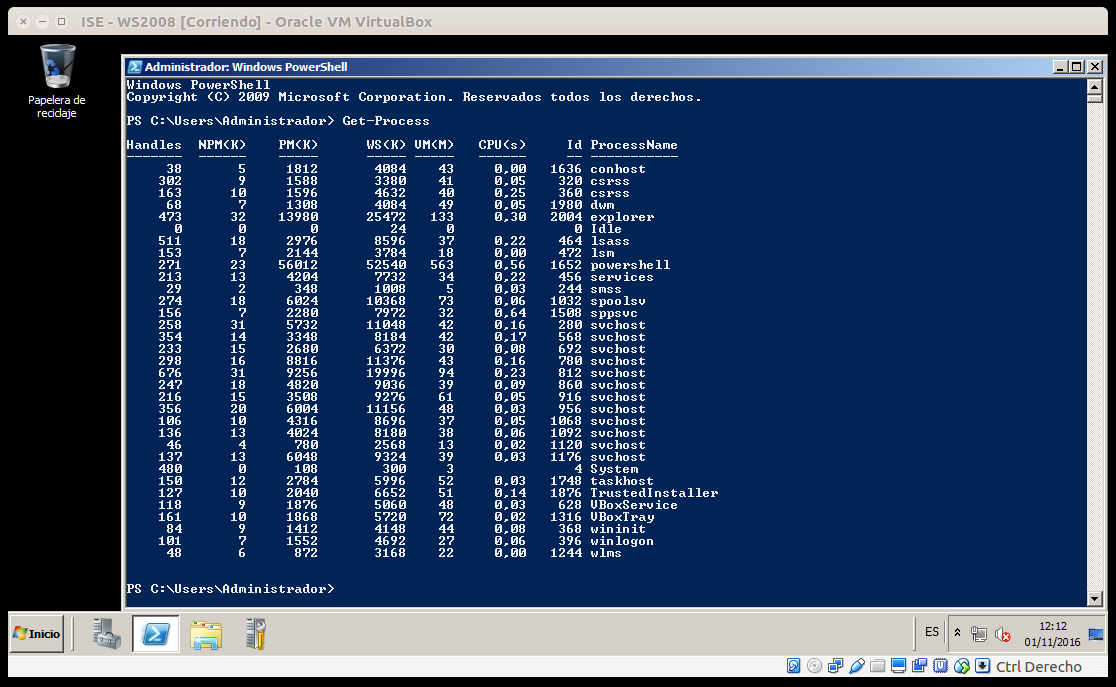
\includegraphics[scale=0.39]{./Imagenes/17-getprocess.png}
		\caption[Procesos activos.]{Procesos activos.}
		\label{17-getprocess}
	\end{figure}
	
	\begin{figure}[H]
		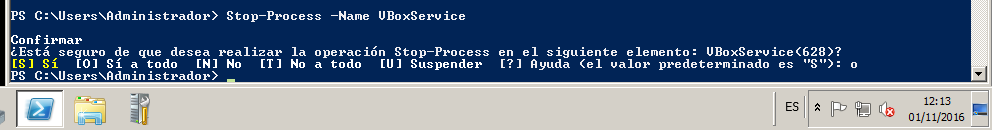
\includegraphics[width=\linewidth]{./Imagenes/17-stopprocess.png}
		\vspace{-0.5cm}
		\caption[Paramos el servicio VBoxService.]{Paramos el servicio VBoxService.}
		\label{17-stopprocess}
	\end{figure}
	
	\begin{figure}[H]
		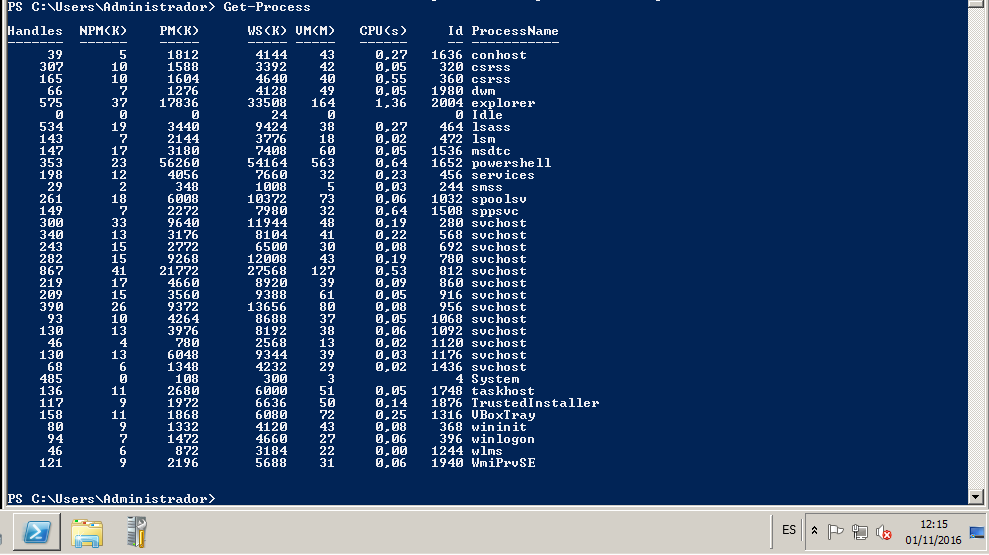
\includegraphics[width=\linewidth]{./Imagenes/17-getprocess2.png}
		\vspace{-0.5cm}
		\caption[Procesos activos tras parar el proceso VBoxService.]{Procesos activos tras parar el proceso VBoxService.}
		\label{17-getprocess2}
	\end{figure}
	
	\clearpage
	
	%%%%%%%%%%%%%%%%%%%%%%%%%%%%%%%%%%%%%%%%%%%%%%%%%%%%
	%%%%%%%%%%%%%%%%%%%% Cuestión Opcional 1 %%%%%%%%%%%
	%%%%%%%%%%%%%%%%%%%%%%%%%%%%%%%%%%%%%%%%%%%%%%%%%%%%
	\section[Cuestión opcional 1: Instale y pruebe terminator y/o tmux. Con screen, pruebe su funcionamiento dejando sesiones ssh abiertas en el servidor y recuperándolas posteriormente.]{Cuestión opcional 1: Instale y pruebe terminator y/o tmux. Con screen, pruebe su funcionamiento dejando sesiones ssh abiertas en el servidor y recuperándolas posteriormente.}
	
	Para instalar \textit{terminator} debemos ejecutar \textit{sudo apt install terminator}. Para instalar \textit{screen} debemos ejecutar \textit{sudo apt install screen}. Aprender a usar \textit{terminator}, a un nivel suficiente para la realización de este ejercicio, es fácil. Pero para aprender a usar \textit{screen} he consultado las páginas del manual \cite{screen}. \\
	
	\begin{enumerate}
		\item Lo primero que he hecho ha sido crear tres terminales en \textit{terminator}, dos para usar \textit{screen} y realizar dos conexiones ssh a mi servidor y una tercera para comprobar el estado de las dos anteriores. En las dos terminales superiores que se ven en la figura \ref{O1-1} he abierto dos sesiones de \textit{screen}. Para ello he ejecutado \textit{screen -S ssh1} en la terminal de la izquierda y \textit{screen -S ssh2} en la terminal de la derecha. Para corroborar que estamos en \textit{screen}, he ejecutado en ambas \textit{echo \$TERM} y efectivamente podemos ver que estamos en screen mientras que en la terminal inferior no. También podemos ver en la terminal inferior como hay dos sesiones de \textit{screen} abiertas. En las terminales superiores he realizado dos conexiones ssh, y he ejecutado dos comandos para ver que, efectivamente, funcionan. Todo este proceso se puede ver en la igura \ref{O1-1}.
		\item A continuación, cerramos \textit{terminator}. Lo abrimos de nuevo y creamos las mismas tres terminales. Podemos comprobar que no estamos en una sesión de \textit{screen} ejecutando \textit{echo \$TERM} y vemos que no estamos en una sesión de \textit{screen}. Para restaurar las sesiones, ejecutamos \textit{screen -r 9417.ssh2} y \textit{screen -r 9403.ssh1}, como podemos ver en la figura \ref{O1-2}.
		\item Tras ejecutar los dos comandos anteriores, podemos ver que se restauran las sesiones de \textit{screen} y las conexiones ssh. Una vez más ejecutamos \textit{echo \$TERM} para ver que, correctamente, estamos en las sesiones de \textit{screen}. Todo este proceso lo podemos ver en la figura \ref{O1-3}.
		\item Para cerrar la sesión de \textit{screen} ejecutamos \textit{exit} dos veces, la primera de ellas para cerrar la conexión ssh y la segunda para cerrar la conexión de \textit{screen}. Finalmente, ejecutamos de nuevo \textit{echo \$TERM} para ver que no estamos en una sesión de \textit{screen}. En la terminal inferior ejecutamos \textit{screen -ls} para ver que no queda ninguna sesión de \textit{screen} abierta. Todo lo comentado podemos verlo en la figura \ref{O1-4}.
	\end{enumerate}
	
	\begin{figure}[H]
		\centering
		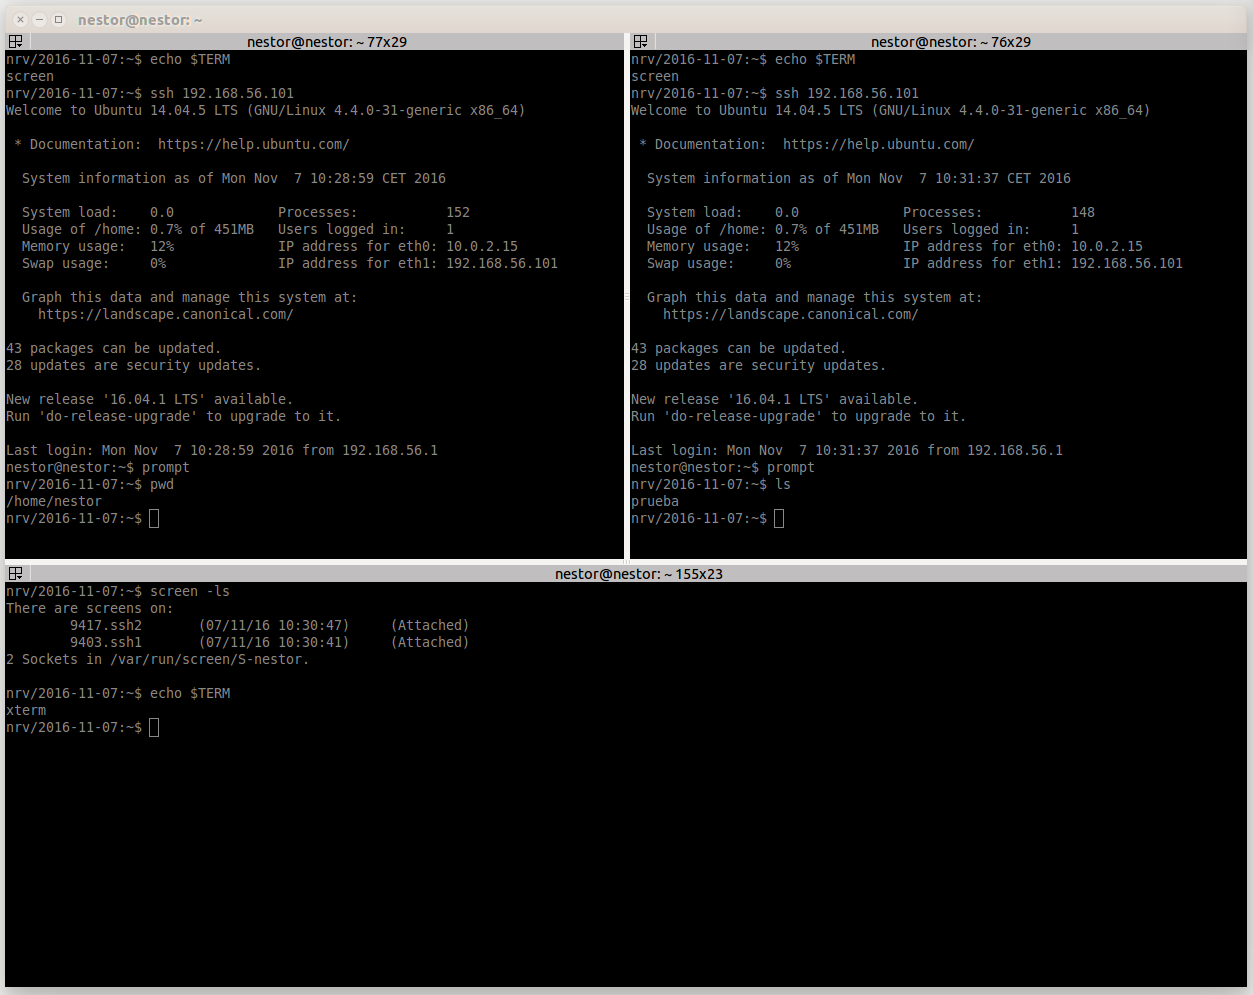
\includegraphics[scale=0.29]{./Imagenes/O1-1.png}
		\caption[Creación de las sesiones de \textit{screen}.]{Creación de las sesiones de \textit{screen}.}
		\label{O1-1}
	\end{figure}
	
	\begin{figure}[H]
		\centering
		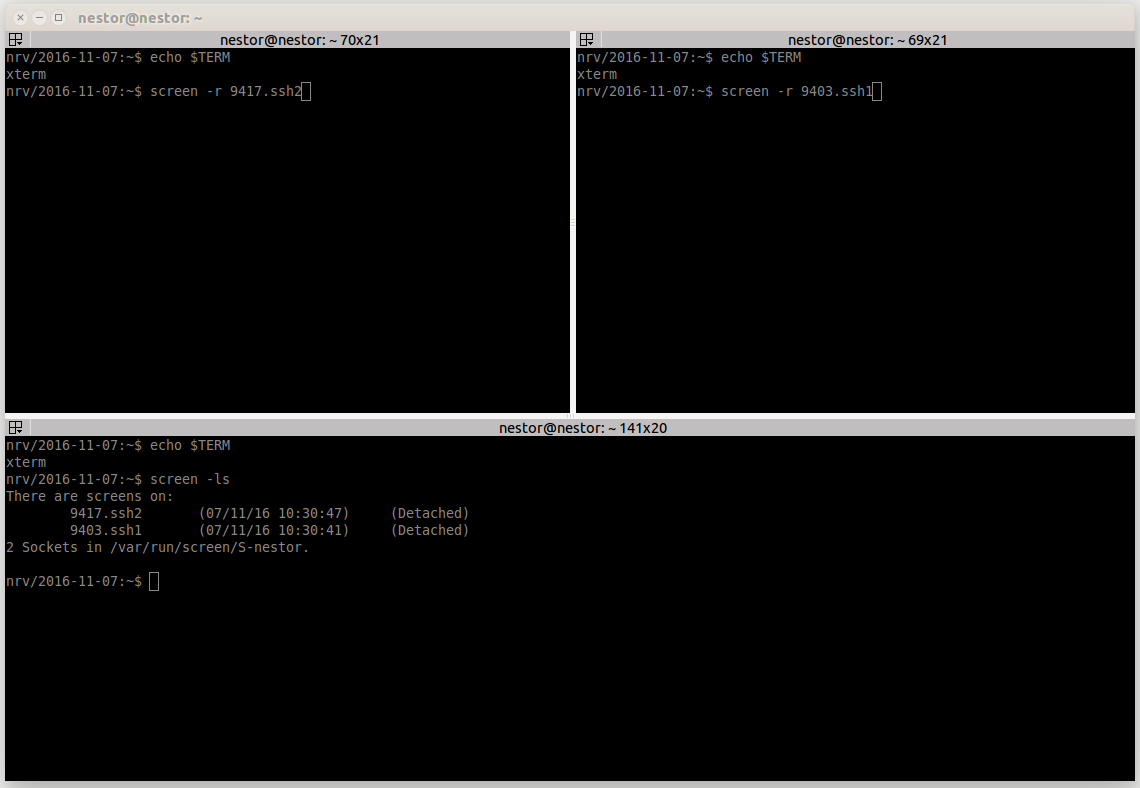
\includegraphics[scale=0.32]{./Imagenes/O1-2.png}
		\caption[Restauración de las sesiones de \textit{screen}.]{Restauración de las sesiones de \textit{screen}.}
		\label{O1-2}
	\end{figure}
	
	\begin{figure}[H]
		\centering
		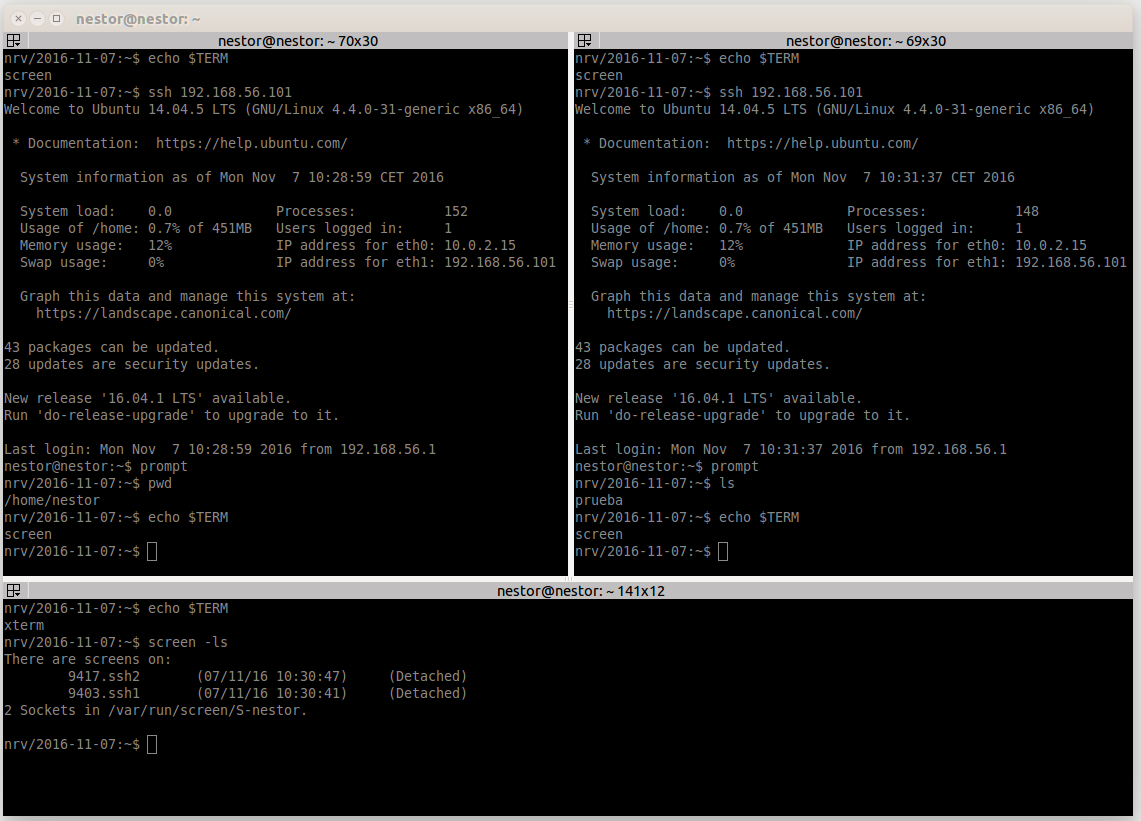
\includegraphics[scale=0.31]{./Imagenes/O1-3.png}
		\caption[Sesiones de \textit{screen} restauradas.]{Sesiones de \textit{screen} restauradas.}
		\label{O1-3}
	\end{figure}
	
	\begin{figure}[H]
		\centering
		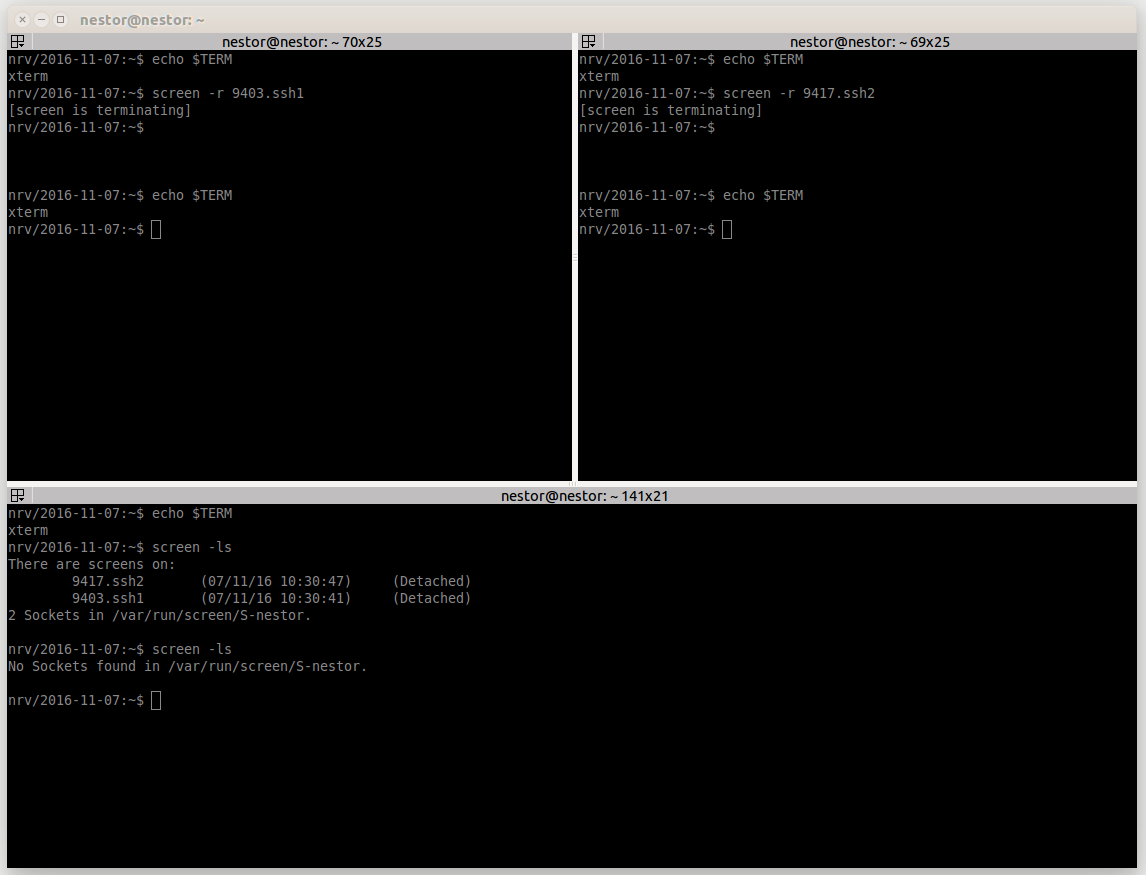
\includegraphics[scale=0.31]{./Imagenes/O1-4.png}
		\caption[Sesiones de \textit{screen} cerradas.]{Sesiones de \textit{screen} cerradas.}
		\label{O1-4}
	\end{figure}
	
	%%%%%%%%%%%%%%%%%%%%%%%%%%%%%%%%%%%%%%%%%%%%%%%%%%%%
	%%%%%%%%%%%%%%%%%%%% Cuestión Opcional 2 %%%%%%%%%%%
	%%%%%%%%%%%%%%%%%%%%%%%%%%%%%%%%%%%%%%%%%%%%%%%%%%%%
	\section[Cuestión opcional 2: Instale el servicio y pruebe su funcionamiento.]{Cuestión opcional 2: Instale el servicio y pruebe su funcionamiento.}
	
	Para ver el funcionamiento de \textit{fail2ban} podemos visitar la página oficial de dicho servicio \cite{fail2ban}. Como página complementaria voy a usar Digital Ocean \cite{fail2bandigitalocean}. Para instalar \textit{fail2ban} debemos ejecutar el comando \textit{sudo apt install fail2ban}. Una vez instalado, lo recomendable es copiar el archivo \textit{/etc/fail2ban/jail.conf} para evitar problemas en futuras actualizaciones. Para ello, ejecutamos el comando \textit{sudo cp /etc/fail2ban/jail.conf /etc/fail2ban/jail.local}, como podemos ver en la figura \ref{O2-copiarjail}.
	\begin{figure}[H]
		\centering
		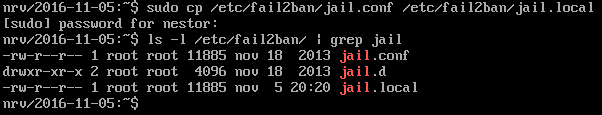
\includegraphics[scale=0.53]{./Imagenes/O2-copiarjail.png}
		\caption[Copia del archivo \textit{/etc/fail2ban/jail.conf}.]{Copia del archivo \textit{/etc/fail2ban/jail.conf}.}
		\label{O2-copiarjail}
	\end{figure}
	
	Para ver su funcionamiento, voy a intentar conectarme a mi servidor \textit{ssh} pero fallaré la contraseña para ver que \textit{fail2ban} funciona correctamente. Como en mi máquina anfitriona tengo configurado \textit{ssh} para permitir el acceso sin contraseña, voy a realizar el intento de acceso desde CentOS, como podemos ver en la figura \ref{O2-accesomal}.
	\begin{figure}[H]
		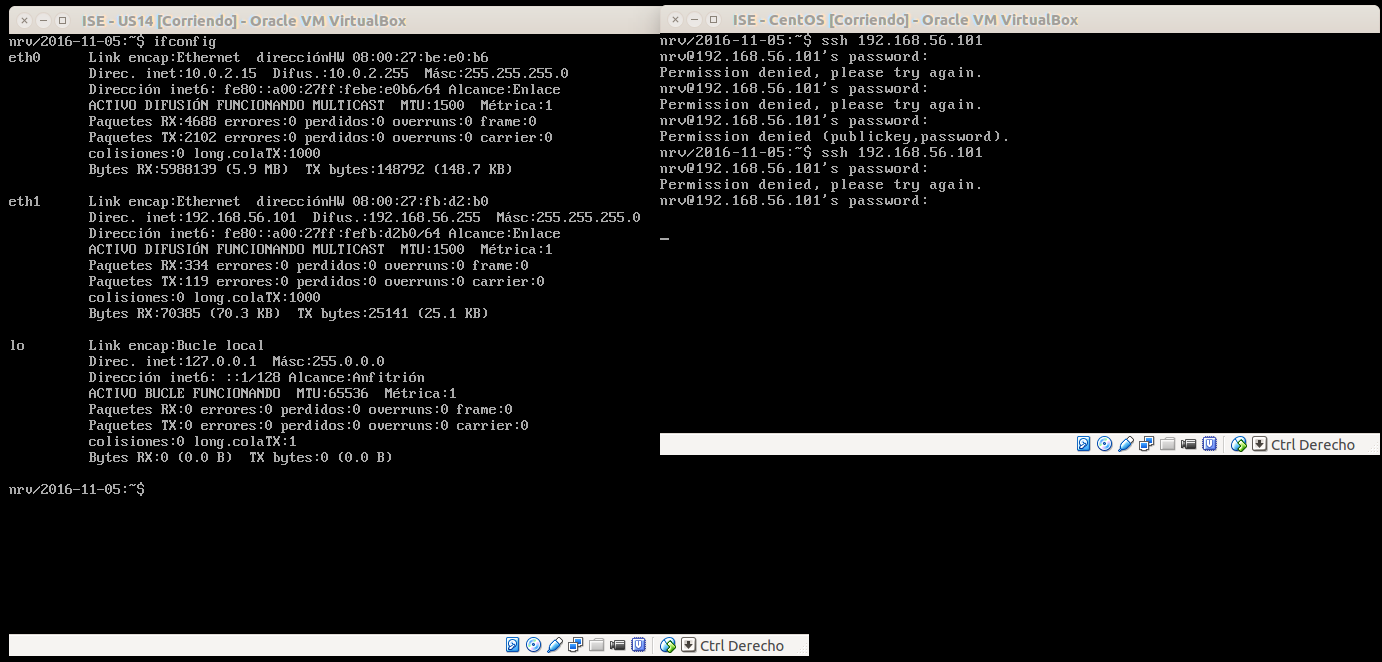
\includegraphics[width=\linewidth]{./Imagenes/O2-accesomal.png}
		\vspace{-0.5cm}
		\caption[Acceso incorrecto (máquinas conectadas en modo \textit{host-only}).]{Acceso incorrecto (máquinas conectadas en modo \textit{host-only}).}
		\label{O2-accesomal}
	\end{figure}
	
	Desde nuestro servidor, ejecutando el comando \textit{sudo iptables -S} vemos que se ha bloqueado la conexión ssh para la IP \textit{} que es la IP de mi máquina virtual de CentOS, como podemos ver en la figura \ref{O2-iptables}.
	\begin{figure}[H]
		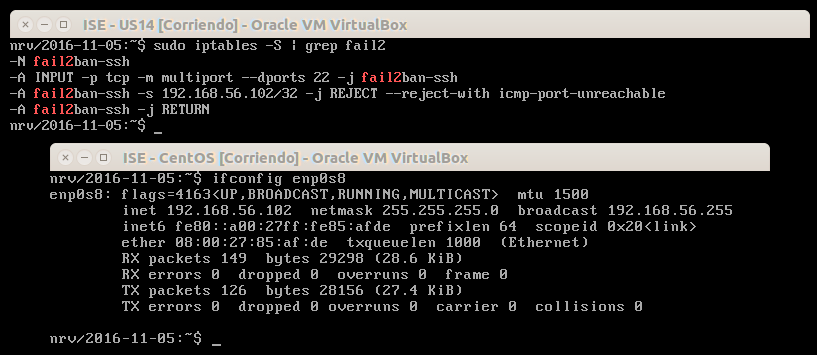
\includegraphics[width=\linewidth]{./Imagenes/O2-iptables.png}
		\vspace{-0.5cm}
		\caption[Dirección IP bloqueada (máquinas conectadas en modo \textit{\textbf{bridge}}).]{Dirección IP bloqueada (máquinas conectadas en modo \textit{\textbf{bridge}}).}
		\label{O2-iptables}
	\end{figure}
	
	%%%%%%%%%%%%%%%%%%%%%%%%%%%%%%%%%%%%%%%%%%%%%%%%%%%%
	%%%%%%%%%%%%%%%%%%%% Cuestión Opcional 3 %%%%%%%%%%%
	%%%%%%%%%%%%%%%%%%%%%%%%%%%%%%%%%%%%%%%%%%%%%%%%%%%%
	\section[Cuestión opcional 3: Instale el servicio y pruebe su funcionamiento.]{Cuestión opcional 3: Instale el servicio y pruebe su funcionamiento.}
	
	Para ver el funcionamiento de \textit{rkhunter} podemos visitar la página oficial de dicho servicio \cite{rkhunter}. Para instalar el servicio ejecutamos \textit{sudo apt install rkhunter}. Lo primero que hacemos es crear una base de datos de como se encuentra nuestro sistema en el momento actual, para luego usarla como referencia. Para ello ejecutamos el comando \textit{sudo rkhunter {-}-propupd}, como podemos ver en la figura \ref{O3-propupd}.
	\begin{figure}[H]
		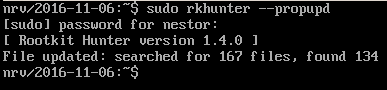
\includegraphics[width=\linewidth]{./Imagenes/O3-propupd.png}
		\vspace{-0.5cm}
		\caption[Creación de la base de datos para \textit{rkhunter}.]{Creación de la base de datos para \textit{rkhunter}.}
		\label{O3-propupd}
	\end{figure}
	
	Una vez hemos creado la base de datos, podemos analizar nuestro sistema ejecutando \textit{sudo rkhunter -c {-}-enable all}. Una vez acabado el análisis, podemos ver un resumen del análisis, como podemos ver en la figura \ref{O3-analisis}.
	\begin{figure}[H]
		\centering
		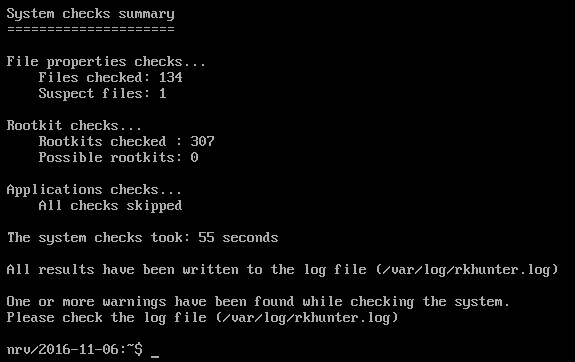
\includegraphics[scale=0.75]{./Imagenes/O3-analisis.png}
		\caption[Resultado del análisis del sistema con \textit{rkhunter}.]{Resultado del análisis del sistema con \textit{rkhunter}.}
		\label{O3-analisis}
	\end{figure}
	
	Como podemos ver en la figura \ref{O3-analisis}, si queremos ver el resultado completo debemos ver el contenido del archivo \textit{/var/log/rkhunter.log}. Finalmente, si queremos actualizar la base de datos que creamos anteriormente, debemos ejecutar el comando \textit{sudo rkhunter {-}-update}
	
	%%%%%%%%%%%%%%%%%%%%%%%%%%%%%%%%%%%%%%%%%%%%%%%%%%%%
	%%%%%%%%%%%%%%%%%%%% Cuestión Opcional 4 %%%%%%%%%%%
	%%%%%%%%%%%%%%%%%%%%%%%%%%%%%%%%%%%%%%%%%%%%%%%%%%%%
	\section[Cuestión opcional 4: Realice la instalación de uno de estos dos “web containers” y pruebe su ejecución.]{Cuestión opcional 4: Realice la instalación de uno de estos dos “web containers” y pruebe su ejecución.}
	
	Voy a probar Apache Tomcat \cite{apachetomcat} en Ubuntu Server. Para instalar Apache Tomat, primero debemos ver si tenemos instalado Java instalado. Para ello, ejecutamos el comando \textit{java -version}. Como podemos ver en la figura \ref{O4-javaversion} Java no se encuentra instalado, para instalarlo ejecutamos \textit{sudo apt-get install default-jdk}
	\begin{figure}[H]
		\includegraphics[width=\linewidth]{./Imagenes/O4-javaversion.png}
		\vspace{-0.5cm}
		\caption[Java no se encuentra instalado de Ubuntu Server.]{Java no se encuentra instalado de Ubuntu Server.}
		\label{O4-javaversion}
	\end{figure}
	
	Una vez hemos instalado java, ejecutamos \textit{sudo apt install tomcat7} para instalar Apache Tomcat. Para ver su funcionamiento, desde la máquina anfitriona vamos a un navegador y escribimos la dirección IP de nuestro servido web seguido de \textit{:8080}. En mi caso, como podemos ver en la figura \ref{O4-ip}, la dirección IP de mi servidos es \textit{192.168.56.101}, por lo tanto en el navegador debemos ir a la dirección \textit{192.168.56.101:8080}. Como podemos ver en la figura \ref{O4-tomcat}, el servicio funciona correctamente.
	\begin{figure}[H]
		\centering
		\includegraphics[scale=0.6]{./Imagenes/O4-ip.png}
		\caption[Dirección IP de mi servidor.]{Dirección IP de mi servidor.}
		\label{O4-ip}
	\end{figure}
	
	\begin{figure}[H]
		\includegraphics[width=\linewidth]{./Imagenes/O4-tomcat.png}
		\vspace{-0.5cm}
		\caption[Servicio \textit{tomcat} funcionando correctamente (máquinas conectadas en modo \textit{host-only}).]{Servicio \textit{tomcat} funcionando correctamente (máquinas conectadas en modo \textit{host-only}).}
		\label{O4-tomcat}
	\end{figure}

	Para acceder al gestor de aplicaciones, como podemos ver en la página de Apache Tomcat \cite{apachetomcatmanager} debemos acceder a la dirección \textit{192.168.56.101:8080/manager/html}. Una vez en esa dirección, nos pide un usuario y una contraseña. Para acceder he creado un usuario con los roles que se puede ver en la figura \ref{O4-tomcat2} y he accedido con el. Dentro de tomcat podemos ver que se puede gestionar diferentes parámetros, como puede ser el tiempo que tardará en expirar una sesión inactiva, como se puede ver en la figura \ref{O4-tomcat2}.
	
	\begin{figure}[H]
		\includegraphics[width=\linewidth]{./Imagenes/O4-tomcat2.png}
		\vspace{-0.5cm}
		\caption[Sesión iniciada en \textit{tomcat} (máquinas conectadas en modo \textit{host-only}).]{Sesión iniciada en \textit{tomcat} (máquinas conectadas en modo \textit{host-only}).}
		\label{O4-tomcat2}
	\end{figure}
	
	%%%%%%%%%%%%%%%%%%%%%%%%%%%%%%%%%%%%%%%%%%%%%%%%%%%%
	%%%%%%%%%%%%%%%%%%%% Cuestión Opcional 5 %%%%%%%%%%%
	%%%%%%%%%%%%%%%%%%%%%%%%%%%%%%%%%%%%%%%%%%%%%%%%%%%%
	\section[Cuestión opcional 5: Realice la instalación de MongoDB en alguna de sus máquinas virtuales. Cree una colección de documentos y haga una consulta sobre ellos.]{Cuestión opcional 5: Realice la instalación de MongoDB en alguna de sus máquinas virtuales. Cree una colección de documentos y haga una consulta sobre ellos.}
	
	Voy a instalar MongoDB en CentoOS. Para ello voy a seguir los pasos de la documentación oficial \cite{mongodb}.
	\begin{enumerate}
		\item Creamos el archivo \textit{/etc/yum.repos.d/mongodb-org-3.2.repo} y añadimos las siguientes líneas:
		\begin{lstlisting}[frame=single, xleftmargin=0.5cm, basicstyle=\footnotesize, label={scriptcrontab}]
[mongodb-org-3.2]
name=MongoDB Repository
baseurl=https://repo.mongodb.org/yum/redhat/$releasever/mongodb-org/3.2/x86_64/
gpgcheck=1
enabled=1
gpgkey=https://www.mongodb.org/static/pgp/server-3.2.asc
		\end{lstlisting}
		El resultado de este paso lo podemos ver en la figura \ref{O5-1}.
		\item Instalamos MongoDB ejecutando \textit{sudo yum install -y mongodb-org}, como podemos ver en la figura \ref{O5-1}.
	\end{enumerate}
	
	Una vez instalado, debemos cambiar el valor de \textit{SELINUX}. Para ello editamos el fichero \textit{/etc/selinux/config} y cambiamos el valor de \textit{SELINUX} a \textit{permissive}, como podemos ver en la figura \ref{O5-2}. Una vez cambiado, debemos reiniciar CentOS. \footnote{Se podría usar \textit{setenforce} pero el cambio no sería permanente.} 
	
	\begin{figure}[H]
		\includegraphics[width=\linewidth]{./Imagenes/O5-1.png}
		\vspace{-0.5cm}
		\caption[Instalación de \textit{MongoDB}.]{Instalación de \textit{MongoDB}.}
		\label{O5-1}
	\end{figure}
	
	\begin{figure}[H]
		\includegraphics[width=\linewidth]{./Imagenes/O5-2.png}
		\vspace{-0.5cm}
		\caption[Cambio de \textit{SELINUX}.]{Cambio de \textit{SELINUX}.}
		\label{O5-2}
	\end{figure}
	
	Para entrar en MongoDB ejecutamos \textit{mongo}. Una vez dentro de MongoDB seguimos los siguientes pasos:
	\begin{enumerate}
		\item Creamos la colección que vamos a usar, \textit{Opcional5\_ISE}, para ello ejecutamos \\ \textit{db.createCollection(`Opcional5\_ISE')}.
		\item Creamos dos documentos para luego insertarlos en la colección que hemos creado en el paso anterior. Para ello ejecutamos:
		\begin{enumerate}
			\item \textit{doc = \{ name: ``Nestor'', age: 20 \}}
			\item \textit{doc2 = \{ name: ``NestorJunior'', age: 10 \}}
		\end{enumerate}
		\item Insertamos los documentos en la colección \textit{Opcional5\_ISE}. Para ello ejecutamos:
		\begin{enumerate}
			\item \textit{db.Opcional5\_ISE.insert(doc)}
			\item \textit{db.Opcional5\_ISE.insert(doc2)}
		\end{enumerate}
		\item Finalmente realizamos la consulta en la colección ejecutando \textit{db.Opcional5\_ISE.find()}
	\end{enumerate}
	
	El resultado de este proceso lo podemos ver en la figura \ref{O5-3}.
	
	\begin{figure}[H]
		\includegraphics[width=\linewidth]{./Imagenes/O5-3.png}
		\vspace{-0.5cm}
		\caption[Creación de la colección, inserción de documentos y consulta.]{Creación de la colección, inserción de documentos y consulta.}
		\label{O5-3}
	\end{figure}
	
	\clearpage
	\bibliography{bibliografia}
	\bibliographystyle{ieeetr}
\end{document}